\chapter{Exemplos de Aplicação}
\label{cap:resultados}

\lstdefinelanguage{NetLogo}{
	morekeywords=[1]{to,to-report,end, extensions,to-report,globals,breed,directed-link-breed, link-breed},
	extendedchars=true, 
    breaklines=true,
    breakatwhitespace=true,
    basicstyle=\ttfamily,
    columns=fullflexible,
	tabsize=4,
    keywordstyle=[1]\color[rgb]{0.25,0.5,0.35},%\color[rgb]{0.4,0.8,0.2}\bfseries,
    morekeywords=[2]{let,set,loop, if, report, foreach, print, tick, while, every, ifelse, ask},
    keywordstyle=[2]\color{blue},
    alsoletter={-,?,.},
    morekeywords=[3]{position, not, reverse, fput, substring, length, word, timer,is-number?,filter,first, bf, butfirst, last, empty?, n-of, color, who, shape},
    keywordstyle=[3]\color[rgb]{0.6,0,0.8},
    comment=[l]{\;},
    commentstyle=\color[rgb]{0.75,0.75,0.75},
    string=[d]{"},
    stringstyle=\color{orange},
    otherkeywords={1, 2, 3, 4, 5, 6, 7, 8, 9, 0},
    morekeywords=[4]{1, 2, 3, 4, 5, 6, 7, 8, 9, 0, true, false},
    keywordstyle=[4]{\color{orange}},
}


Este capítulo apresenta uma primeira aplicação da abordagem proposta no capítulo anterior para o projeto de sistemas de inteligência ambiental (sistemas \acrshort{ami}). Conforme mencionado, a abordagem consiste em uma contribuição para a etapa de análise funcional do sistema e no \textit{feedback} que ela pode dar para refinar a análise de requisitos e a síntese do projeto. O domínio de aplicação da ideia escolhido pertence à área de pesquisa e desenvolvimento tecnológico resultante da combinação da robótica autônoma e da inteligência ambiental, mais especificamente o campo dos robôs aspiradores de pó.

Apesar do domínio de aplicação específico, como o mundo dos aspiradores de pó, o capítulo visa mostrar aos projetistas de sistemas \acrshort{ami} em geral, como projetar estes sistemas em termos de modelos \acrshort{fec} associados e como realizar estudos experimentais objetivando verificar/encontrar decomposições funcionais alternativas de subsistemas componentes capazes de atender aos requisitos funcionais e de desempenho dos sistemas \acrshort{ami}. O ambiente de tarefas, os programas dos agentes representando as pessoas e os robôs aspiradores de pó foram implementados em NetLogo \cite{wilensky1999netlogo}, uma plataforma de \textit{software} que facilita o desenvolvimento das capacidades dos programas dos agentes e do dinamismo do ambiente. A razão para a escolha dessa plataforma é a alta simplicidade em representar os agentes, facilitando a construção de ambientes complexos em curto espaço de tempo. Os códigos utilizados para construir a simulação podem ser observados no seguinte endereço \footnote{https://bitbucket.org/rob\_oliveira/netlogocleanersim}.

O capítulo foi dividido em mais quatro seções. A Seção \ref{sec:dom-aplicacao} descreve o domínio de aplicação, isto é, o sistema \acrshort{ami} pretendido e seu ambiente de tarefas. A Seção \ref{sec:cenario-teste} apresenta o cenário de teste adotado, as propriedades do ambiente de tarefas e as funcionalidades necessárias ao sistema neste ambiente. A Seção \ref{sec:plat-sim} apresenta os principais aspectos associados à plataforma de simulação NetLogo, que são importantes para a compreensão dos resultados. A Seção \ref{sec:dev-experimento} apresenta os projetos em modelos \acrshort{fec} e os resultados (objetos emergentes) de suas simulações na NetLogo. E, finalmente, na seção \ref{sec:conclusao}, discutimos os resultados obtidos nos experimentos. 

\section{Domínio de Aplicação}
\label{sec:dom-aplicacao}

O domínio proposto está dentro de uma combinação das áreas de robótica autônoma e de inteligência ambiental. De um lado, a robótica autônoma visando criar robôs compostos por sensores, atuadores e controladores, que sejam capazes de viver em casas e locais públicos, e sejam habilidosos na realização de tarefas físicas que ajudem na vida cotidiana das pessoas. De outro lado, a inteligência ambiental visando criar redes de dispositivos domésticos inteligentes capazes de fornecer informações, comunicação e serviços para as pessoas. A Figura \ref{fig:dom-ami} ilustra um exemplo desses robôs autônomos em um ambiente de computação ubíqua inteligente, em que existem muitos computadores e redes sensores no ambiente para a geração de informações úteis para o controle dos robôs.

\begin{figure}[h!]
    \centering
    \Caption{\label{fig:dom-ami} Ilustração da ideia de inteligência ambiental e robôs autônomos} 
    \UECEfig{}{
        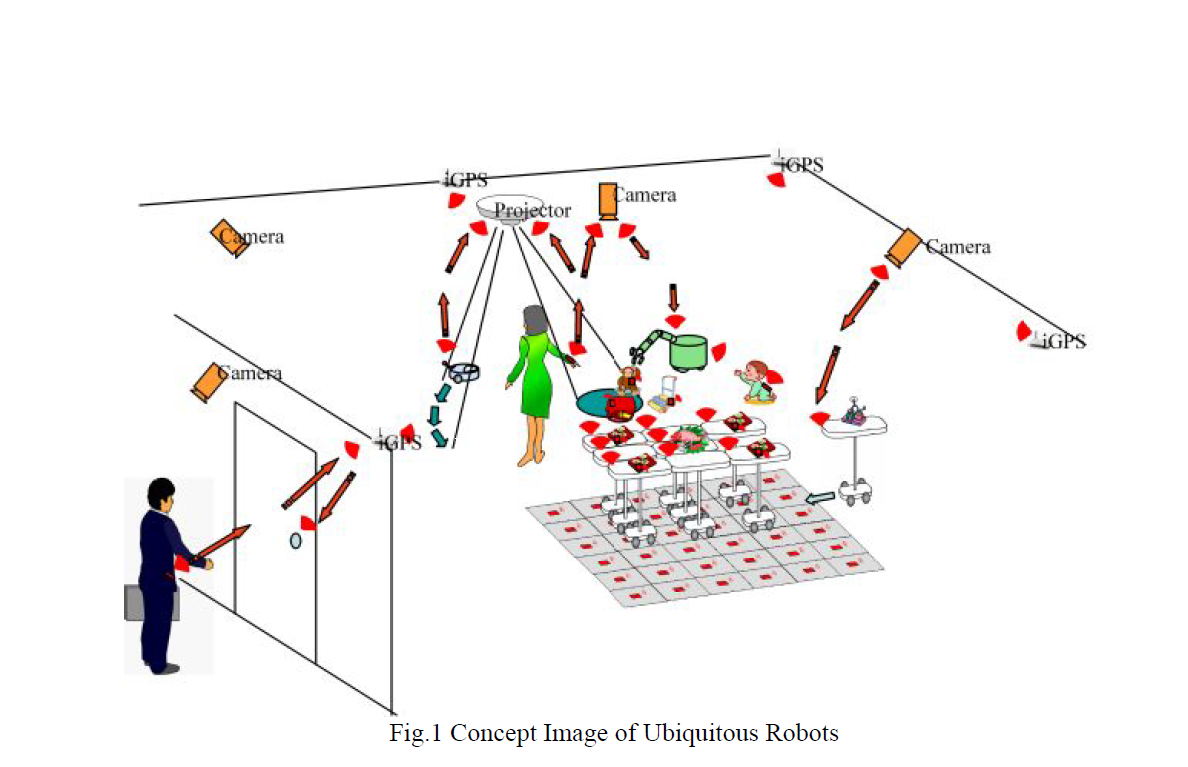
\includegraphics[width=8cm]{figuras/dom-ami}
    }{
        \Fonte{Elaborada pelo autor}
    }   
\end{figure}

Dentro do contexto da combinação da robótica autônoma e da inteligência ambiental, o sistema \acrshort{ami} para aplicação da abordagem envolve o campo dos robôs aspiradores de pó. Este tipo de robô faz parte do mundo atualmente conhecido como Internet das Coisas (\acrshort{iot}). O propósito de um robô aspirador é ser um servo para as pessoas, economizando o tempo e esforço, limpando a sujeira de locais de interesse. Por exemplo, a fabricante LG disponibiliza uma vasta gama de aparelhos inteligentes que são controlados por um aplicativo de mensagens. Em particular, tal empresa fabrica um robô aspirador denominado \textit{HomeBot Square}  (Figura \ref{fig:cleaner-bot}a). Através do aplicativo de mensagens, o \textit{HomeBot Square} e outros dispositivos inteligentes LG podem ser programados com comandos em linguagem natural.

\begin{figure}[h!]
    \centering
    \Caption{\label{fig:cleaner-bot} Aspiradores de pó inteligentes: HomeBot Square e Roomba 980} 
    \UECEfig{}{
        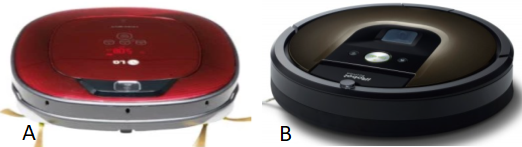
\includegraphics[width=8cm]{figuras/cleaner-bot.png}
    }{
        \Fonte{Elaborada pelo autor}
    }   
\end{figure}

A companhia iRobot fabrica o robô aspirador Roomba 980 (Figura \ref{fig:cleaner-bot}b). Conhecido como o aspirador da Internet das Coisas, o Roomba 980 pode ser controlado por meio de aplicativos. A companhia garante que o robô é capaz de executar suas tarefas em um tempo contínuo de duas horas, retornando automaticamente à sua base de carga e em seguida voltar ao trabalho até que o local pretendido esteja limpo. Roomba é capaz de limpar área abertas movendo-se em linhas paralelas, empregando um conjunto de sensores para adaptar este padrão quando necessário, navegando perfeitamente entre os móveis e a desordem. Essencialmente, a iRobot instalou uma câmera em cima do Roomba 980, a qual constantemente mapeia o local à medida que o robô se movimenta, tornando-o mais eficiente. 

\section{Cenário de Teste}
\label{sec:cenario-teste}

Para ilustrar a aplicação da abordagem, o cenário de teste considera um sistema técnico composto por um conjunto de agentes artificiais robôs aspiradores de pó responsáveis por limpar uma área quadrada (retangular) em um aeroporto, que pode conter obstáculos, sujeira e pessoas, distribuídas de maneira aleatória em uma área determinada. A Figura \ref{fig:ami-aplication} ilustra um cenário específico, contendo um conjunto de quatro agentes artificiais, quatro usuários, três obstáculos, três pontos de recarga de energia e bastante lixo. 

\begin{figure}[h!]
    \centering
    \Caption{\label{fig:ami-aplication}Exemplo de um cenário de teste.} 
    \UECEfig{}{
        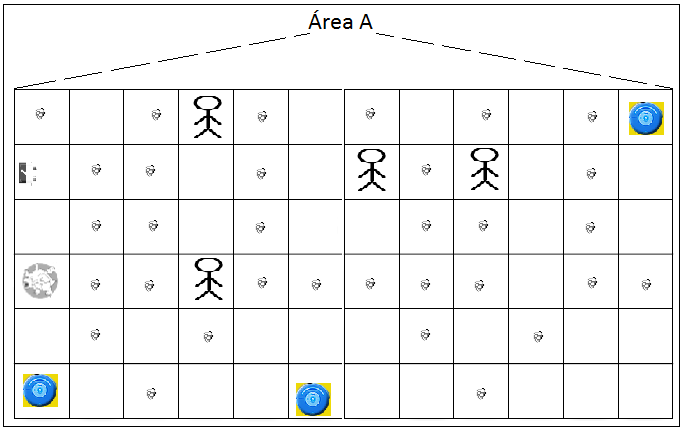
\includegraphics[width=8cm]{figuras/ami-aplication.png}
    }{
        \Fonte{Elaborado pelo autor.}
    }   
\end{figure}

O ambiente de tarefas é parcialmente observável e não determinístico, pois alguns atuadores dos robôs podem falhar. As pessoas que circulam pelo ambiente podem depositar sujeira pelos locais por onde passam, tornando o ambiente dinâmico. Uma configuração particular do ambiente pode ser definida considerando-se as quantidades de robôs, de obstáculos, de lixo e de pessoas em locais específicos do aeroporto. Diferentes configurações compreendem diferentes cenários (casos) de teste, definindo problemas de diferentes níveis de dificuldade. Por exemplo, algumas configurações podem exigir dos robôs maior consumo de energia, enquanto outras podem colocar lixo em locais de mais fácil acesso aos robôs. 

Nesse tipo de ambiente difícil, cada agente artificial aspirador de pó deve ser capaz de perceber e atualizar seu conhecimento sobre o ambiente sempre que se mover, identificando e localizando cada um dos objetos, visando realizar o objetivo original do sistema, ou seja, limpar o máximo de sujeira possível, gastando o mínimo de energia e evitando obstáculos quando for necessário. Ele também deve ser capaz de cooperar com os outros agentes no ambiente, por meio de processos de comunicação e troca de conhecimentos úteis para a realização de seus objetivos e do objetivo original do sistema. A Seção \ref{sec:dev-experimento} descreve em detalhes a funcionalidade de cada um dos agentes no cenário proposto. 


\section{Plataforma de Simulação}
\label{sec:plat-sim}

O ambiente de simulação e os programas dos agentes representando as pessoas e os robôs aspiradores de pó foram implementados em NetLogo \cite{wilensky1999netlogo}, uma plataforma de \textit{software} que facilita o desenvolvimento das capacidades dos programas dos agentes e do dinamismo do ambiente. O ambiente é concebido como um recipiente em que existem objetos observáveis, incluindo obstáculos, lixo e pessoas. As propriedades dos objetos podem ser alteradas e novos objetos podem ser concebidos facilmente e inseridos no ambiente. A Figura \ref{fig:netlogo-env} ilustra um ambiente em tempo de execução. Neste ambiente, existe um agente aspirador de pó (vermelho), cinco obstáculos (marron) e uma grande quantidade de sujeira (cinza).


\begin{figure}[h!]
    \centering
    \Caption{\label{fig:netlogo-env}Simulação NetLogo: programa aspirador de pó em um ambiente de tarefas.} 
    \UECEfig{}{
        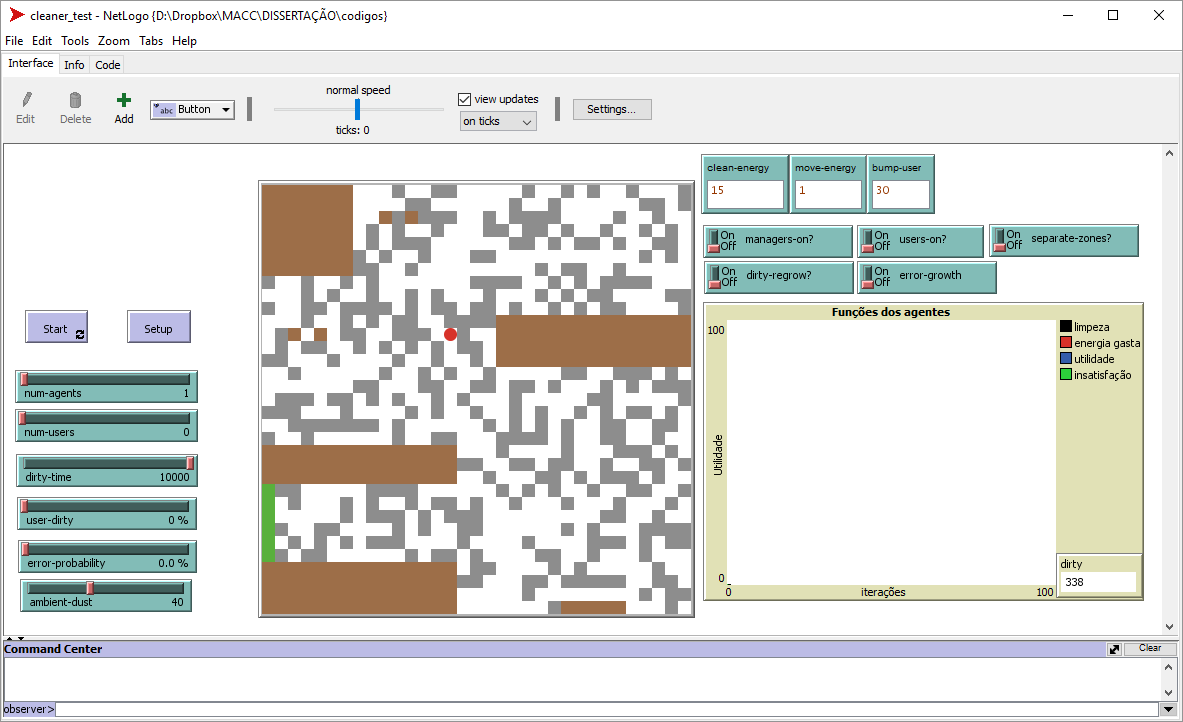
\includegraphics[width=10cm]{figuras/netlogo-env}
    }{
        \Fonte{Elaborado pelo autor}
    }   
\end{figure}

NetLogo disponibiliza uma linguagem de programação com atributos multiagentes. Ela possui capacidades que a tornam muito poderosa, tanto para produzir quanto para visualizar simulações de \acrlong{sma}. NetLogo é implementada em Java, seu código é compacto e simples de compreender, tornando-a ideal para demonstrar ideias complexas de forma sucinta. Além disso permite que os usuários adicionem extensões para a linguagem, criando novos comandos \cite{teahan2010artificial}.

Existem quatro tipos de agentes em NetLogo, são eles: \textit{patches}, \textit{turtles}, \textit{links} e o \textit{observer}. Os agentes \textit{turtles} são capazes de se movimentar e interagir com o ambiente. Os agentes \textit{Patches} representam o ambiente por onde os \textit{turtles} caminham. Em um ambiente bidimensional os \textit{patches} são representados por um \textit{grid}, onde cada célula contém um \textit{patch}. Estes dois tipos são os principais agentes utilizados para construir aplicações. 

Os agentes \textit{links} não possuem uma representação visual, mas simbolizam uma ligação entre dois ou mais agentes \textit{turtles}. O agente \textit{observer} é o agente gestor, capaz de controlar toda a aplicação, não sendo permitido ao usuário utilizá-lo. Ele também não possui uma representação visual, e é usado para adicionar, ou remover, entidades da aplicação além de observar seu comportamento. 

\section{Projetando o sistema AmI}
\label{sec:dev-experimento}

O objetivo desta seção consiste em apresentar a aplicação da abordagem proposta em cenários de teste semelhantes aos descritos na Seção \ref{sec:cenario-teste}. A apresentação é realizada em diversas subseções. Cada subseção foi dividida em duas partes. A primeira apresenta o modelo \acrshort{fec} associado a uma organização de programas de agentes empregada para representar um sistema técnico, composto por um ou mais robôs aspiradores, e as pessoas no ambiente de tarefas. A segunda parte apresenta os objetos emergentes resultantes de simulações considerando diferentes configurações do ambiente de tarefas, ou seja, fixando-se dimensões e obstáculos, variando-se a quantidade de sujeira, o número de pessoas usuárias, e os tipos de robôs aspiradores no ambiente.

As subseções componentes foram organizadas em uma sequência tal que os detalhes da aplicação do modelo \acrshort{fec} são apresentados evolutivamente. A Subseção \ref{subsec:exp1} considera um sistema \acrshort{ami} composto por um único sistema técnico, ou seja, um único robô aspirador, que interage com um ambiente de tarefas contendo apenas sujeira e obstáculos. A Subseção \ref{sec:exp-dinamico} modifica o ambiente, tornando ele dinâmico, e adiciona um elemento não determinístico ao comportamento do aspirador. A seção \ref{sec:exp-user} adiciona a entidade usuário a simulação. Na seção \ref{sec:multi-asp} observamos o comportamento do sistema quando um conjunto de aspiradores são inseridos no ambiente. A seção \ref{sec:exp-coord} adiciona uma outra entidade, chamada coordenador, que tem o objetivo de controlar as ações dos aspiradores. E finalmente, na seção \ref{sec:grupo}, dividimos os agentes da simulação em grupos no ambiente.

\subsection{Sistema \textit{AmI} com um único sistema técnico em um ambiente sem pessoas}
\label{subsec:exp1}

O primeiro experimento considera um sistema \acrshort{ami} com um sistema técnico formado por um único robô aspirador em um ambiente de tarefas que consiste em um certo local em um aeroporto. A Figura \ref{fig:ambiente-exp1} ilustra um ambiente representado por uma grade de $32 \times 32$ \textit{patches}. Os obstáculos (marrom) e a sujeira (cinza) são os únicos objetos observáveis no ambiente. O aspirador (vermelho) deve e realizar o objetivo original ($O_O$) do sistema \acrshort{ami} em um horário em que não existem pessoas transitando. 

\begin{figure}[h!]
    \centering
    \Caption{\label{fig:ambiente-exp1}Sistema \textit{AmI} aspirador único em ambiente sem pessoas.} 
    \UECEfig{}{
        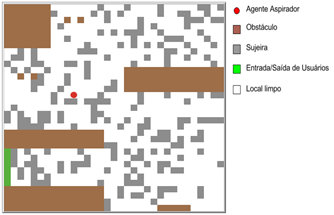
\includegraphics[width=10cm]{figuras/exp1-amb22}
    }{
        \Fonte{Elaborado pelo autor}
    }   
\end{figure}

O agente aspirador se movimenta pelo local visando limpar toda a sujeira nele contida. Ele deve evitar colisão com os obstáculos e procurar minimizar o gasto de energia. O ambiente é parcialmente observável e determinístico. As simulações das interações do sistema técnico com o ambiente consideram diversos cenários diferentes quanto à quantidade e distribuição inicial de sujeira, mas idênticos quanto à posição dos obstáculos no ambiente. 

\subsubsection{Modelo F}

A Figura \ref{fig:arq-agent-amb} ilustra a relação agente-ambiente, empregando o termo $AgentAmI$ para representar o programa de agente $AgSoftware$ componente do sistema técnico, cujo \textit{hardware} é formado por um sensor e um atuador. A figura ilustra também outros termos empregados na concepção do quadro formal que define o modelo $F$. Em qualquer instante $k$ o sensor do aspirador percebe ($s^{*k}$) uma grade de $32 \times 32$ \textit{patches}, os quais podem ser do tipo limpo, sujo ou obstáculo, e o seu atuador executa uma ação adequada ($a^{*k}$) entre aquelas que são possíveis de serem executadas pelo aspirador.

\begin{figure}[h!]
    \centering
    \Caption{\label{fig:arq-agent-amb}– Interações do programa AgentAmi no ambiente Amb.} 
    \UECEfig{}{
        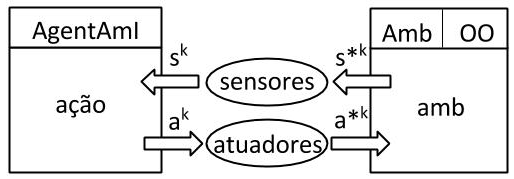
\includegraphics[width=6cm]{figuras/arq-agent-amb.png}
    }{
        \Fonte{Elaborado pelo autor}
    }   
\end{figure}

A figura identifica um episódio $Ep^K$ do programa $AgentAmI$ concebido para realizar o objetivo original $O_O$ no ambiente de tarefas $Amb$, tal que:

\begin{itemize}
    \item $S = \{s^1, s^2, \ldots \}$ -- Estados do ambiente –- em qualquer instante $k$ o sensor do aspirador disponibiliza um estado $s^k$ consistindo de uma grade menor, contida na grade $32\times32$ \textit{patches} que representa o local, de tamanho $3\times3$ \textit{patches}, ou seja, o conjunto de estados do ambiente é formado por todas as grades desse tamanho, em que cada \textit{patch} pode representar uma parte limpa (branco) ou suja (cinza) do local, ou a presença de um obstáculo (marrom) na parte;
    
    \item $A = \{a^1, a^2, \ldots \}$ -- Capacidade efetuadora -– em qualquer instante $k$ o atuador do aspirador consegue executar uma ação $a^k$ que pode ser: locomover-se do \textit{patch} em que o aspirador está para outro \textit{patch}, em qualquer direção (norte, sul, leste, oeste), ou limpar o \textit{patch} em que o aspirador está (aspirar);   
    
    \item ação:$S^*  \rightarrow A $ -- Comportamento -– função para seleção de ações em $A$ adequadas aos estados em $S$, ou seja, o aspirador deve aspirar em \textit{patches} cinza, e deve mudar para um \textit{patch} vizinho que seja cinza se estiver em um \textit{patch} branco;
    
    \item amb: $S\times A \rightarrow S$ -- Comportamento (determinístico) ambiente –- função para mudança de estados do ambiente de acordo com as ações executadas pelo agente – se o aspirador limpar em um \textit{patch} cinza então este deve mudar para branco, e se o aspirador seguir de um \textit{patch} para outro em uma determinada direção então mudar posição do agente para este outro \textit{patch}; 
    
    \item AgentAmI -- Um programa de agente implementando concretamente em linguagem NetLogo a função ação de um agente aspirador;
    
    \item Amb -- Um programa ambiente implementando concretamente em linguagem NetLogo a função amb;

    
    \item $\Omega$ -- Um conjunto formado por todas as grades de tamanho $32 \times 32$ \textit{patches}, diferentes quanto a quantidade de \textit{patches} do tipo cinza;
    
    \item $Cenario_i \in \Omega$ -- Uma grade de tamanho $32 \times 32$ \textit{patches}, os quais podem ser do tipo branco, cinza ou marrom; 
    
    \item $Cenario_i \in P(\Omega)$ -- Um subconjunto formado por $10 (N_{Cenarios})$ grades de $32 \times 32$ \textit{patches}, os quais podem ser do tipo branco, cinza ou marrom;
    
    \item $h(Cenario_i) \in (S\times A)^{Nint}$ -- Uma história formada por 100 ($NInt$) de $AgentAmI$ em $Amb$ correspondente ao $Cenario_i \in \Omega$; 
    
    \item $Ep^k(h(Cenario_i)) \in (S\times A)$ -- Um episódio na interação k, $k \leq 10$, da história de $AgentAmI$ em $Amb$ correspondente ao caso $Cenario_i \in \Omega$;
    
    \item $H(Cenario_i)) \in P((S\times A)^{Nint})$ -- Um conjunto de 10 histórias de comprimento 100 de $AgentAmI$ em $Amb$;
    
\end{itemize}

Neste experimento, o objetivo original ($O_O$) do sistema consiste em prestar um serviço de alta qualidade com um mínimo de despesas no ambiente. O modelo $F$ aplicado propõe definir formalmente $O_O$ por meio de uma função de utilidade, a qual considera um vetor de duas funções ($f_1$ e $f_2$) objetivos próximos ($O_1$ e $O_2$) de $O_O$, as quais têm o mesmo valor de importância no contexto de $O_O$, e são expressas em termos de duas funções escalares ($av_1$ e $av_2$), associadas aos atributos de descrição de estados, ou seja, a limpeza do ambiente e a quantidade de energia utilizada. A Tabela \ref{tab:objetivo-exp1} coloca em destaque os dois objetivos próximos e a notação empregada para as funções objetivos e escalares associadas.

\begin{table}[h!]   
    \centering
    \Caption{\label{tab:objetivo-exp1} Objetivos próximos do objetivo original.}
    \UECEtab{}{
        \begin{tabular}{cccc}
            \toprule
                Objetivo &  Descrição   &   Função Objetivo & Recompensa \\
                \midrule \midrule
                $O_1$  & Manter o ambiente limpo & $f_1(H(Cenarios))$ & $av_1(Ep^k(h(Cenario_i)))$ \\
                $O_2$  & Manter energia na bateria & $f_2(H(Cenarios))$ & $av_2(Ep^k(h(Cenario_i)))$ \\
            \bottomrule
        \end{tabular}
    }{
    \Fonte{Elaborado pelo autor}
}
\end{table}
    
Cada uma das funções escalares, $av_1$ e $av_2$, associa valores no domínio dos números reais, ou seja, valores de satisfação/insatisfação nos objetivos próximos $O_1$ e $O_2$, com um conjunto de episódios possíveis $(Ep(s,a) \in S\times A)$, descritos em termos de um conjunto de estados do ambiente ($s \in S$) e um conjunto de ações possíveis para o aspirador ($a \in A$). Abaixo a definição formal das funções escalares empregadas neste experimento:

\[
av_1(Ep((s^k, a^k)) =
\begin{cases}
  15 & \text{se $s^k$ = cinza e $a^k$ = aspirar,}\\
  0 & \text{se $s^k$ = branco e $a^k$ = aspirar,}\\
  0 & \text{se $s^k$ = cinza ou branco e $a^k$ = norte ou sul ou leste ou oeste}
\end{cases}
\]

e, 

\[
av_2(Ep((s^k, a^k)) =
\begin{cases}
  2 & \text{se $s^k$ = cinza ou branco e $a^k$ = aspirar,}\\
  1 & \text{se $s^k$ = cinza ou branco e $a^k$ = norte ou sul ou leste ou oeste}
\end{cases}
\]

Consequentemente, as funções objetivos podem ser definidas para para um conjunto formado por 10 cenários de teste ($N_{Cenarios}$ = 10), cada cenário associado a uma história formada por 100 episódios ($N_{Int}$ = 100) de interação do aspirador no ambiente:

\[
    f_1(H(\textrm{Cenários}))=\frac{1}{10}\sum_{i=1}^{10}Av_1(h(Cenario_i))
\]
e,
\[
    f_2(H(\textrm{Cenários}))=\frac{1}{10}\sum_{i=1}^{10}Av_2(h(Cenario_i)),
\]

tal que:

\[
Av_1(h(\textrm{Cenário}_i)) =  \sum_{k=1}^{100}av_1(Ep((s^k, a^k))
\]

e, 

\[
Av_2(h(\textrm{Cenário}_i)) = \sum_{k=1}^{100}av_2(Ep((s^k, a^k))
\]

E, finalmente, considerando-se que os dois objetivos próximos têm o mesmo valor de importância, a função utilidade para medir o alcance do objetivo original pelo aspirador pode ser definida.

\[ U(f(H(Cenarios)) = f_1(H(Cenarios)) - f_2(H(Cenario))\]

Assim, se o aspirador de pó for capaz de maximizar a função utilidade, isto é, se ele for capaz de maximizar a quantidade de patches limpos em 100 interações, minimizando o gasto de energia, então será adequado ao seu ambiente de tarefas, pois é capaz de realizar os objetivos próximos com os quais está comprometido e, consequentemente, de satisfazer o objetivo original do sistema.

\subsubsection{Modelo E}

O termo $AgentAmI$ na Figura \ref{fig:arq-agent-amb} foi empregado para representar o componente de \textit{software}, ou seja, um programa de agente do tipo $AgSoftware$, do sistema técnico aspirador de pó, o qual tem como componentes de \textit{hardware} um sensor e um atuador. Assim, de acordo com as propostas $P_2$ e $P_3$ na abordagem, este primeiro experimento considerou dois programas de agente do tipo $AgHardware$, um capaz de simular a realização do processamento de informações perceptivas ($s^{*k}$) realizado pelo sensor e outro para simular a execução de ações ($a^{*k}$) pelos atuadores do aspirador. A Figura \ref{fig:exp1-modelE} esboça os programas e a maneira como estão organizados na representação do sistema AmI.

\begin{figure}[h!]
    \centering
    \Caption{\label{fig:exp1-modelE}Organização de programas de agentes representando o robô aspirador.} 
    \UECEfig{}{
        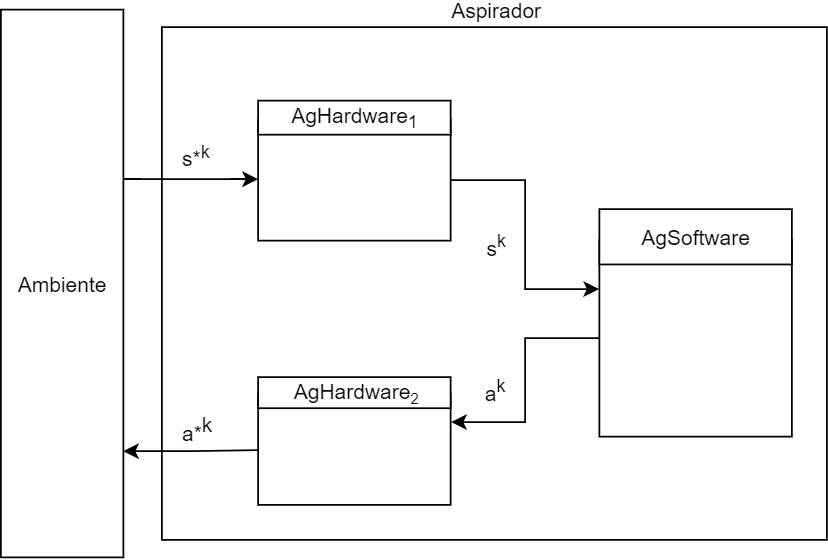
\includegraphics[width=6cm]{figuras/exp1-aspirador-modelE.png}
    }{
        \Fonte{Elaborado pelo autor}
    }   
\end{figure}

Os dois programas de agente $AgHardware_1$ e $AgHardware_2$ representam respectivamente o sensor e o atuador do sistema técnico no ambiente. O programa $AgSoftware$ processa as informações perceptivas oriundas do processamento do programa $AgHardware_1$, seleciona ações e envia para o programa $AgHardware2$, o qual deve executar estas ações no ambiente.

Quanto ao modelo $E$ associado à figura, consiste na definição dos conjuntos de programas de agentes e de papéis que os programas podem assumir na organização, das relações entre os papéis, dos grupos de programas e da cardinalidade destes grupos, ou seja: 

\begin{itemize}
    \item $Agents$ --	$\{AgHardware_1, AgHardware_2, AgSoftware\}$ – conjunto de três ($N_A = 3$) programas $AgentAmI$ na organização.
    
    \item $Roles$ -- $\{Device, Controller\}$ – conjunto de dois ($N_R = 2$) papéis que podem ser atribuídos aos programas de agentes $AgentAmI$.
    
    \item $AgentsRoles$ -- $\{AgentAmIDevice, AgentAmIController\}$ – família de dois ($N_R = 2$) conjuntos, tal que:
    
    \begin{itemize}
        \item $AgentAmIDevice$ -- $\{AgHardware_1, AgHardware_2\}$ – conjunto de programas no papel \textit{Device};
        \item $AgentAmIController$ -- $\{AgSoftware\}$ – conjunto de programas no papel \textit{Controller}.
    \end{itemize}
    
    \item $Bond$ -- \{$Bond_{knowledge}(AgentAmIDevice, AgentAmIController)$, 
                    \\$Bond_{knowledge}(AgentAmIController, AgentAmIDevice)$,
                    \\$Bond_{\textrm{Coordenação}}(AgentAmIDevice, AgentAmIController)$, 
                    \\$Bond_{\textrm{Coordenação}}(AgentAmIController, AgentAmIDevice)$\} – família de quatro relações entre os programas nos conjuntos $AgentAmIDevice$ e $AgentAmIController$, tal que:
    \begin{itemize}
        
        \item $Bond_{knowledge}(AgentAmIDevice, AgentAmIController)$ --	\{$(AgHardware_1, AgSoftware), \\(AgHardware_2, AgSoftware)$\} – programas $AgHardware_1$ e $AgHardware_2$ (papel \textit{Device}) têm o conhecimento da existência do programa $AgSoftware$ (papel \textit{Controller});
        
        \item $Bond_{knowledge}(AgentAmIController, AgentAmIDevice)$ -- \{$(AgSoftware$, $AgHardware_1$), ($AgSoftware$, $AgHardware_2$)\} – programa $AgSoftware$ tem o conhecimento da existência dos programas $AgHardware_1$ e $AgHardware_2$;
        
        \item $Bond_{\textrm{Coordenação}}(AgentAmIDevice, AgentAmIController)$ -- \{($AgHardware_1$, $AgSoftware$\} – cada ato de informação do programa $AgHardware_1$ ao programa AgSoftware gera o conhecimento correspondente no programa AgSoftware;
        
        \item $Bond_{\textrm{Coordenação}}(AgentAmIController, AgentAmIDevice)$ -- \{($AgSoftware$, $AgHardware_2$)\} – cada ato de informação do programa $AgSoftware$ ao programa $AgHardware_2$ gera o conhecimento correspondente no programa $AgHardware_2$
        .
    \end{itemize}
    
    \item $Groups$ --\{$AgHardware_1$, $AgHardware_2$, $AgSoftware$\} – família de um ($N_G = 1$) conjunto de programas de agentes exercendo seus papéis na organização.
    
    \item $Communication$ -- \{($AgHardware_1$, $AgSoftware$), ($AgSoftware$, $AgHardware_2$)\} – relação descrevendo quem pode enviar mensagens para quem na organização;
    
    \item $Frequency$ -- Figura \ref{fig:exp1-matriz-socio} – matriz sociométrica informa a frequência com que os programas de agentes trocam mensagens entre si.
    
\end{itemize}
    
    Os dois últimos itens descrevem a segunda parte do modelo. A Figura \ref{fig:exp1-matriz-socio} define a matriz sociométrica de acordo com o ponto de vista do projetista. Esta matriz permite ao projetista definir o mapa das interações que ocorrem entre os programas de agentes em diferentes papéis dentro dos grupos que compõem a organização. 
    
    \begin{figure}[h!]
        \centering
        \Caption{\label{fig:exp1-matriz-socio}Matriz sociométrica.} 
        \UECEfig{}{
            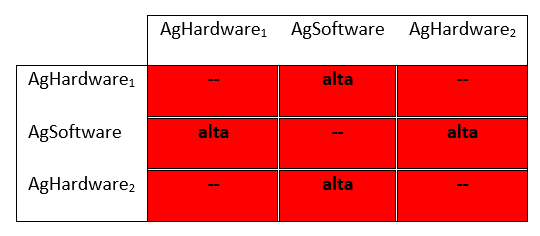
\includegraphics[width=6cm]{figuras/exp1-matriz-socio}
        }{
            \Fonte{Elaborado pelo autor}
        }       
    \end{figure}
    
    Por exemplo, A matriz sociométrica acima informa que a frequência \emph{freq($AgHardware_1$, \\AgSoftware)} com que o par de programas de agentes $(AgHardware_1, AgSoftware) \in Communication$ troca mensagens entre si é alta. A matriz informar estas concentrações de interações densas neste único grupo, de forma que as células com os maiores de valores de frequência ficaram ao longo da diagonal principal, e todos as células fora destes quadrados da diagonal têm valores de frequência zero.

\subsubsection{Modelo C}

O modelo comportamental descreve como a estrutura projetada deve funcionar para realizar o objetivo original do sistema, sua função descrita no modelo $F$, no ambiente de tarefas. O modelo de C neste primeiro experimento consiste na descrição formal dos procedimentos de tomada de decisão nos três programas de agentes em seus papéis na organização, $Agents = \{AgHardware_1, AgHardware_2, AgSoftware\}$, e dos processos que ocorrem dentro da organização, isto é, como os três programas de agentes integrados na estrutura organizacional devem agir.

No que diz respeito aos procedimentos de tomada de decisão, os “esqueletos” dos programas representando o agente aspirador de pó na Figura \ref{fig:exp1-modelE}, os programas $AgHardware_1$ e $AgHardware_2$, no papel $Device$ no modelo $E$, são do tipo reativo simples, e o programa $AgSoftware$, no papel $Controller$ no modelo $E$, também do tipo reativo. A Figura \ref{fig:exp1-modelC-detail} ilustra a customização dos esqueletos dos programas representando o agente artificial aspirador de pó único, interagindo com um ambiente que representa um local onde não existem pessoas transitando.

\begin{figure}[h!]
    \centering
    \Caption{\label{fig:exp1-modelC-detail}Esqueletos dos programas de agentes representando o sistema AmI.} 
    \UECEfig{}{
        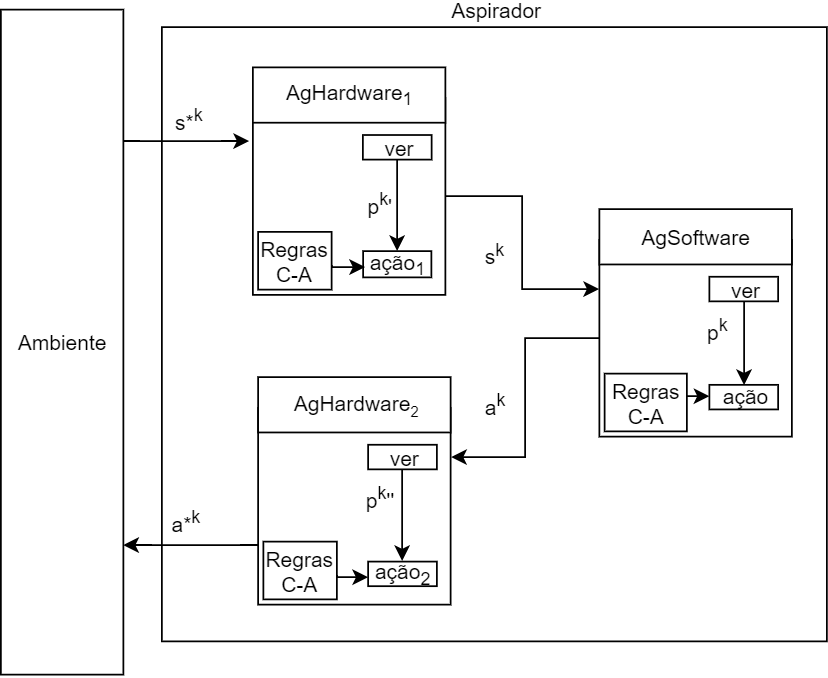
\includegraphics[width=10cm]{figuras/exp1-aspirador-G.png}
    }{
        \Fonte{Elaborado pelo autor}
    }   
\end{figure}

Estendendo-se o quadro desenvolvido no modelo $F$ para os três programas de agentes reativos, têm-se que:
\begin{itemize}
    \item $S^* = \{s^{*1}, s^{*2}, \ldots\}$ -- Estados do ambiente – em qualquer instante $k$ o programa $AgHardware_1$, representando o sensor do aspirador, percebe um estado $s^{*k}$ consistindo de uma grade de $32 \times 32$ \textit{patches} que representa uma parte do ambiente.
    
    \item $P_1 = \{p^{1\prime}, p^{2\prime}, \ldots \}$ -- Percepção do programa $AgHardware_1$ – 
    em qualquer instante $k$ o programa $AgHardware_1$ ao receber do ambiente entradas perceptivas $s^{*k} \in S^*$ – estados do 
    ambiente consistindo de uma grade de tamanho $32 \times 32$ 
    \textit{patches} – representa estas informações em uma linguagem interna adequada $p^{k\prime} \in P_1$.
    
    \item $ver_1: S^*  \rightarrow P_1$ --	Subsistema de percepção de $AgHardware_1$ – mapeia estados $s^{*k} \in S^*$ para percepções na linguagem interna $p^{k\prime} \in P_1$.
    
    \item $\textrm{ação}_1: P_1 \rightarrow S$ -- Subsistema de tomada de decisão de $AgHardware_1$ – função que mapeia percepções na linguagem $p^{k\prime} \in P_1$ em entradas perceptivas $s^k \in S$ – estados do ambiente consistindo de uma grade de tamanho $3 \times 3$ \textit{patches} – enviadas para o programa $AgSoftware$.
    
    \item $P = \{p^1, p^2, \ldots \}$ -- Percepção do programa $AgSoftware$ – em qualquer instante $k$ o programa $AgSoftware$ ao receber do programa $AgHardware_1$ as entradas perceptivas $s^k \in S$ – estados do ambiente consistindo de uma grade de tamanho $3 \times 3$ \textit{patches} – representa estas informações em uma linguagem interna adequada $p^k \in P$.
    
    \item $ver: S  \rightarrow P$ -- Subsistema de percepção de $AgSoftware$ – mapeia estados $s^k \in S$ para percepções na linguagem interna $p^k \in P$.
    
    \item $\textrm{ação}: P \rightarrow A$ -- Subsistema de tomada de decisão de $AgSoftware$ – função que mapeia percepções na linguagem $p^k \in P$ em descrições de ações $a^k \in A$ – locomover-se de um \textit{patch} para outro vizinho, em qualquer direção (norte, sul, leste, oeste), ou limpar o \textit{patch} em que o aspirador está (aspirar) – enviadas para o programa $AgHardware_2$.
    
    \item $P_2 = \{p^{1\prime\prime}, p^{2\prime\prime}, \ldots\}$	Percepção do programa $AgHardware_2$ – em qualquer instante $k$ o programa $AgHardware_2$ ao receber de $AgSoftware$ descrições de ações $a^k \in A$, representa estas informações em uma linguagem interna adequada $p^{k\prime\prime} \in P_2$.
    
    \item $ver_2: A  \rightarrow P_2$ -- Subsistema de percepção de $AgHardware_2$ – mapeia descrições de ações $a^k \in A$ para percepções em uma linguagem interna adequada $p^{k\prime\prime} \in P_2$.
    
    \item $\textrm{ação}_2: P_2 \rightarrow A$ -- Subsistema de tomada de decisão de $AgHardware_2$ – função que mapeia percepções na linguagem $p^{k\prime\prime} \in P_2$ em ações $a^{*k} \in A$ – locomover-se de um \textit{patch} para outro vizinho, em qualquer direção (norte, sul, leste, oeste), ou limpar o \textit{patch} em que o aspirador está (aspirar).
    
\end{itemize}

O conjunto de regras C-A do agente $AgHardware_1$ busca representar a noção de ambiente parcialmente observável pelo sensor do aspirador de pó, determinando a redução na quantidade de informações a respeito do ambiente presente em $p^{k\prime} \in P_1$, isto é, estados consistindo de uma grade de tamanho $32 \times 32$ \textit{patches} descritos na linguagem interna de $AgHardware_1$. Estas regras, orientam as ações deste programa, isto é, entradas perceptivas $s^k \in S$, neste experimento uma redução para uma grade de tamanho $3 \times 3$ \textit{patches}, enviadas para o programa $AgSoftware$. As regras C-A do $AgHarware_2$, neste momento, não interferem nas ações do agente  $Agsoftware$, ou seja, $a^{*k} = a^k \in A$.

O conjunto de regras C-A que orientam a seleção de ações adequadas à percepção $p^{k\prime\prime} \in P_2$, gerada na linguagem interna de $AgSoftware$ a partir das entradas perceptivas $s^k \in S$, geradas por $AgHardware_1$ e enviadas para o programa $AgHarware_2$, ou seja: locomover-se de um \textit{patch} para outro vizinho, em qualquer direção (norte, sul, leste, oeste), ou limpar o \textit{patch} em que o aspirador está. O algoritmo \ref{alg:exp1-behaviour} ilustra o conjunto de regras C-A incorporado no programa AgSoftware.

\begin{algorithm}[h!]
    %\SetSpacedAlgorithm
    \caption{\label{alg:exp1-behaviour} Conjunto de regras condição-ação do programa controlador AgSoftware.}
    %\Entrada{$p^k$ em S}
    %\Saida{$a^k$ em A}
    função ação ($p^k$ em S) retorna $a^k$ em A\\
    \Inicio{
        \ldots\\
        \textbf{se} $p^k$ (grade $3 \times 3$ \textit{patches}) \textit{patch} do aspirador cinza (sujo) \textbf{então} $a^k$ = aspirar\;
        \textbf{se} $p^k$ \textit{patch} do aspirador branco (limpo) e \textit{patch} cinza a norte  \textbf{então} $a^k$ = norte\;
        \textbf{se} $p^k$ \textit{patch} do aspirador branco e \textit{patch} cinza a sul  \textbf{então} $a^k$ = sul\;
        \textbf{se} $p^k$ \textit{patch} do aspirador branco e \textit{patch} cinza a leste  \textbf{então} $a^k$ = leste\;
        \textbf{se} $p^k$ \textit{patch} do aspirador branco e \textit{patch} cinza a oeste  \textbf{então} $a^k$ = oeste\;
        
        \textbf{se} $p^k$ \textit{patch} do aspirador branco e \textit{patch} marrom a norte  \textbf{então} $a^k$ = sul\;
        \textbf{se} $p^k$ \textit{patch} do aspirador branco e \textit{patch} marrom a sul  \textbf{então} $a^k$ = norte\;
        \textbf{se} $p^k$ \textit{patch} do aspirador branco e \textit{patch} marrom a leste  \textbf{então} $a^k$ = oeste\;
        \textbf{se} $p^k$ \textit{patch} do aspirador branco e \textit{patch} marrom a oeste  \textbf{então} $a^k$ = leste\;
        
        \textbf{se} $p^k$ \textit{patch} do aspirador branco e outros \textit{patches} brancos  \textbf{então} $a^k$ = mover-random\;
        
        \ldots\\
    }
\end{algorithm}

O conjunto de regras determina o comportamento do aspirador no ambiente de operação. Conforme indicado na seção que define o Modelo $F$, cada \textit{patch} possui uma cor simbolizando sujeira (ou não) e a presença de obstáculos. Em resumo, sempre que o aspirador estiver sobre um \textit{patch} de cor cinza ele deve selecionar a ação aspirar. Se ele estiver sobre um \textit{patch} branco (limpo) então deverá seguir para o local sujo mais próximo. Se o aspirador não detectar sujeira dentro do perímetro escaneado, ele escolherá de maneira aleatória uma direção para seguir em frente.

O conjunto de regras especificado visa exemplificar a descrição do componente de tomada de decisão do programa $AgSoftware$, por isso não foi detalhado com o rigor necessário para realizar os objetivos próximos do objetivo original, implícitos na função utilidade descrita no modelo $F$ da organização. O conjunto de regras encerra a especificação do modelo $C$ associado ao comportamento do componente de \textit{software} do sistema \acrshort{ami} proposto no primeiro experimento.

Dando continuidade à descrição do modelo $C$, no que diz respeito à sua segunda parte, a Figura \ref{fig:exp1-protocol} descreve o protocolo de interação descrevendo as trocas de mensagens possíveis, no modelo $E$ descritas na relação Communication.

\begin{figure}[h!]
    \centering
    \Caption{\label{fig:exp1-protocol} Protocolo de interação entre os programas na organização.} 
    \UECEfig{}{
        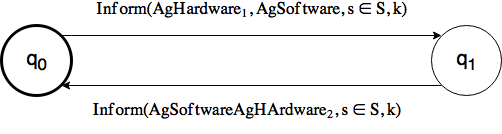
\includegraphics[width=8cm]{figuras/inform-protocol-hard-soft.png}
    }{
        \Fonte{Elaborado pelo autor}
    }   
\end{figure}

A relação $Communication$ descreve quem pode enviar mensagens para quem na organização, $Communication = \{(AgHardware_1, AgSoftware), (AgSoftware, AgHardware_2)\}$. A família de conjuntos de programas que compõem a organização, contém um único conjunto de três agentes, $G = \{{AgHardware_1, AgHardware_2, AgSoftware}\}$. O protocolo considera um conjunto de dois estados possíveis, $Q = \{q_0, q_1\}$. O estado inicial foi representado por $q_0$.

No início da interação, no instante $k$, o agente aspirador de pó percebe seu ambiente de tarefas por meio de seu sensor. Ou seja, o programa ambiente $Amb$ envia a informação $s^* \in S^*$ para o programa $AgHardware_1$, que, depois de processá-la, envia a informação $s \in S$ para o programa $AgSoftware$, isto é, $\delta(q_0, inform(AgHardware_1, AgSoftware, s \in S, k)) = q_1$. Posteriormente, o programa $AgSoftware$ processa essa informação, toma uma decisão e envia uma ação para ser executada no ambiente por um de seus atuadores. Ou seja, no modelo $C$, $AgSoftware$ envia a informação $a \in A$ para o programa $AgHardware_2$, $\delta(q_1, inform(AgHardware_2, AgSoftware, s \in S, k)) = q_0$, que, depois de processá-la, encerra a interação $k$ enviando uma ação $a^* \in A$ para o programa ambiente $Amb$.

Por motivos de simplicidade, a Figura \ref{fig:exp1-protocol} não ilustra as interações entre o aspirador e o seu ambiente de tarefas, isto é, o envio de mensagem contendo informação $s^* \in S^*$ do programa ambiente $Amb$ para o programa sensor $AgHardware_1$, e de mensagem contendo informação $a^* \in A$ do programa atuador $AgHardware_2$ para o programa $Amb$. A figura encerra a especificação do modelo \acrshort{fec} para o sistema \acrshort{ami} formado por um único aspirador em um local em que não existem pessoas transitando. A próxima subseção apresenta os objetos emergentes de interesse associados ao modelo $F$ deste sistema \acrshort{ami}. 

\subsubsection{Objetos Emergentes}

Conforme a Figura \ref{fig:sim-emergente-p6} indica. A simulação do sistema \acrshort{ami} utiliza como informações de entrada o modelo \acrshort{fec} construído para o sistema. Além disso, são utilizados dados do ambiente de tarefas e parâmetros de inicialização da aplicação, para descrever um contexto operacional de funcionamento do sistema no ambiente. Ao executar a simulação com as informações fornecidas, ela deve gerar como saída dados sobre o desempenho do sistema, conforme descrito no modelo $F$. Isto é, os objetos emergentes resultantes das interações descritas no modelo $C$, e da racionalidade das ações selecionadas pelos programas de agentes na organização estruturada no modelo $E$.

Este experimento buscou investigar o desempenho do programa $AgSoftware$, responsável pelo controle do agente artificial aspirador de pó, variando-se a quantidade inicial de sujeira no ambiente. Em um primeiro momento, o agente será inserido em um cenário onde 10\% dos \textit{patches} do ambiente estará sujo. Em cada um dos cenários posteriores a quantidade de \textit{patches} sujos será aumentada em 10\%. Serão ao todo dez cenários analisados, culminando em um cenário onde todos os \textit{patches} disponíveis estão sujos. 

Para cada um dos dez cenários de teste foram realizadas 100 simulações, totalizando mil execuções. A Figura \ref{fig:exp1-sim-exec} ilustra um exemplo da evolução dos valores das funções escalares empregadas neste experimento e da função utilidade, ao longo de 1000 interações do agente com o ambiente em um único cenário ambiental. 

\begin{figure}[h!]
    \centering
    \Caption{\label{fig:exp1-sim-exec} Medidas de desempenho em 1000 interações.} 
    \UECEfig{}{
        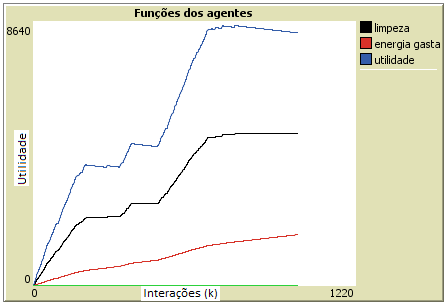
\includegraphics[width=8cm]{figuras/exp1-sim-exec.png}
    }{
        \Fonte{Elaborado pelo autor}
    }   
\end{figure}

A cada simulação executada são observadas informações a respeito dos objetivos próximos definidos no modelo $F$. Os objetivos $O_1$, manter o ambiente limpo, e $O_2$, economizar energia, são associados respectivamente as funções escalares $av_1$ e $av_2$. Essas funções são representadas na Figura \ref{fig:exp1-sim-exec} pelas curvas de limpeza e energia. A função Utilidade, que representa o desempenho do sistema em seu objetivo original $O_O$ (prestar um serviço de alta qualidade com um mínimo de despesas no ambiente), é composta por ambas as funções $av_1$ e $av_2$. Observando o comportamento dessas funções podemos deduzir informações sobre o desempenho do sistema \acrshort{ami}.

Uma coleção destas deduções, obtidas metodicamente pela execução de 100 simulações em cada cenário, permite a realização de inferências sobre o desempenho do sistema, em termos de medidas de distribuições, e se o mesmo será capaz de realizar o objetivo original em seu ambiente de tarefas. As Figuras \ref{fig:exp1-perf-limpeza} e \ref{fig:exp1-perf-utilidade} ilustram estas medidas de distribuições obtidas no primeiro experimento. 

\begin{figure}[h!]
    \centering
    \Caption{\label{fig:exp1-perf-limpeza} Distribuição do objetivo $O_1$.} 
    \UECEfig{}{
        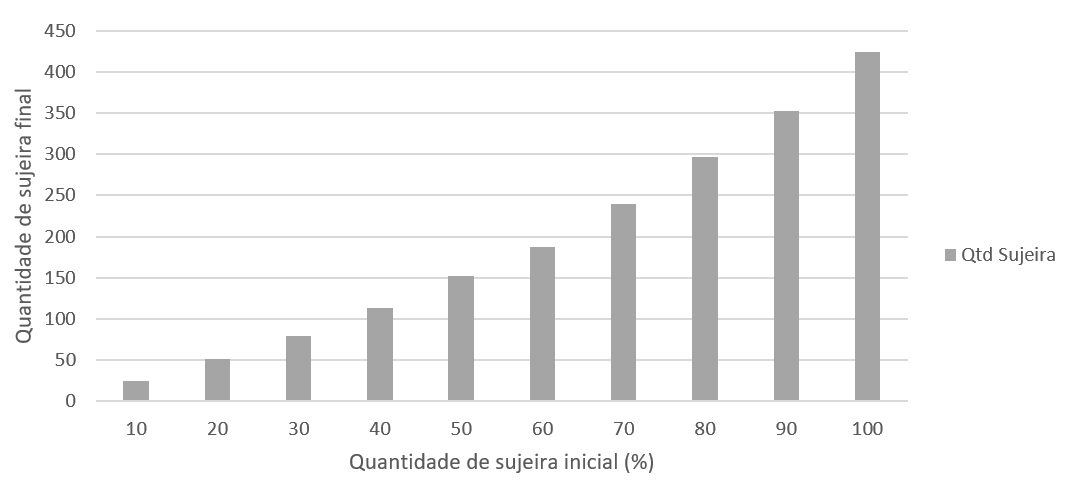
\includegraphics[width=10cm]{figuras/exp1-perf-limpeza.png}
    }{
        \Fonte{Elaborado pelo autor}
    }   
\end{figure}

A Figura \ref{fig:exp1-perf-limpeza} apresenta uma distribuição associada a quantidade de sujeira que permaneceu no ambiente ao fim da simulação. Representando a eficiência do agente em manter o ambiente limpo. Lembrando que medida associada ao objetivo $O_1$ representa a limpeza do ambiente da perspectiva do aspirador e não do ambiente. Não surpreendentemente, os resultados observados em cada um dos cenários caracterizam uma curva que cresce quase que linearmente à medida que aumenta a quantidade inicial de sujeira no ambiente.

\begin{figure}[h!]
    \centering
    \Caption{\label{fig:exp1-perf-utilidade} Distribuição de Utilidade do experimento.} 
    \UECEfig{}{
        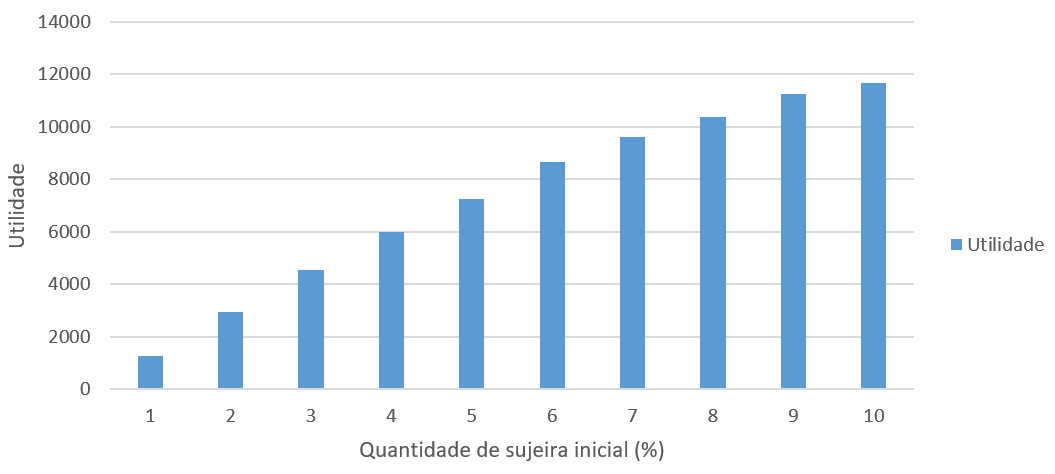
\includegraphics[width=10cm]{figuras/exp1-perf-utilidade.png}
    }{
        \Fonte{Elaborado pelo autor}
    }   
\end{figure}

Por outro lado, a distribuição associada à função utilidade, apresentada na Figura \ref{fig:exp1-perf-utilidade}, segue um padrão quase que logarítmico, tendendo a um valor máximo. Esse comportamento também já era esperado, pois, independente da estratégia de limpeza adotada, o sistema \acrshort{ami} é composto por um único agente aspirador para todo o ambiente. 


\subsection{Sistema \textit{AmI} com um único sistema técnico em um ambiente não determinístico}
\label{sec:exp-dinamico}
Em vez de buscar melhorar o subsistema de tomada de decisão do programa controlador $AgSoftware$ no modelo $C$, nesta segunda parte do experimento vamos “injetar realidade” nas simulações envolvendo o mundo do aspirador de pó único, ou seja, tornando o ambiente dinâmico e não determinístico. Para simular um ambiente dinâmico, periodicamente o programa ambiente $Amb$ deposita sujeira em locais que foram previamente limpos pelo aspirador. Para simular um ambiente não determinístico o programa $AgHardware_2$, representando os atuadores do aspirador, poderá deixar de executar uma ação enviada por AgSoftware, caracterizando uma falha.

A simulação em um ambiente de tarefas não determinístico está relacionada com a proposta \textbf{P7} na abordagem. Especificamente neste experimento o projetista deve entender como os efeitos da aleatoriedade das ações executadas pelos atuadores do aspirador interferem na forma e nas propriedades macro de cada distribuição. Esse entendimento deve servir para garantir que este componente de confiabilidade baixa e integrado no aspirador, não o impedirá de alcançar o objetivo original em um ambiente de tarefas dinâmico. No que diz respeito ao modelo \acrshort{fec} associado ao experimento, somente o modelo $C$ deve ser alterado, mantendo-se os modelos $F$ e $E$ já definidos.

\subsubsection{Modelo C}

No que diz respeito aos procedimentos de tomada de decisão, os “esqueletos” dos programas $AgHardware_1$ e $AgSoftware$, são os mesmos apresentados na Figura \ref{fig:exp1-modelE}  e no resto do modelo $C$ descrito na mesma seção. Somente o esqueleto do programa $AgHadware_2$, no papel \textit{Device} no modelo $E$, deve sofrer alteração. No experimento anterior, as regras C-A do agente $AgHardware_2$ repetiam as ações que eram executadas pelo agente $AgSoftware$.

Neste experimento o programa $AgHardware_2$ será do mesmo tipo, porém, seu conjunto de regras será modificado para simular que os atuadores do aspirador estão sujeitos ao não determinismo. Ou seja, ele pode falhar em executar as ações selecionadas por $AgSoftware$. Mais formalmente em algumas ocasiões pode ser que $a^{*k} \neq a^k \in A$. 

O conjunto de regras C-A no subsistema de tomada de decisão de $AgHarware_2$ implementam as falhas possíveis no atuador do aspirador de pó, isto é, a ação $a^{*k} \in A$ que vai ser executada no ambiente, em função da ação $a^k \in A$ enviada por $AgSoftware$, mais especificamente, da representação desta informação $p^{k\prime\prime} \in P$, gerada na linguagem interna de $AgHardware_2$, e do instante $k$ das interações do aspirador com o seu ambiente. O algoritmo \ref{alg:exp2-behaviour} ilustra o conjunto de regras incorporado no programa $AgHardware_2$.


\begin{algorithm}[h!]
    %\SetSpacedAlgorithm
    \caption{\label{alg:exp2-behaviour} Conjunto de regras condição-ação do programa atuador $AgHardware_2$.}
    %\Entrada{$p^k$ em S}
    %\Saida{$a^k$ em A}
    função ação ($p^{k\prime\prime}$ em P) retorna $a^{*k}$ em A\\
    \Inicio{
        \ldots\\
        \textbf{se} $p^{k\prime\prime}$ = norte e falha(k) \textbf{então} $a^{*k}$ = move-random\;
        \textbf{senão se} $p^{k\prime\prime}$ = norte \textbf{então} $a^{*k}$ = norte\;
        \textbf{se} $p^{k\prime\prime}$ = sul e falha(k) \textbf{então} $a^{*k}$ = move-random\;
        \textbf{senão se} $p^{k\prime\prime}$ = sul \textbf{então} $a^{*k}$ = sul\;
        \textbf{se} $p^{k\prime\prime}$ = leste e falha(k) \textbf{então} $a^{*k}$ = move-random\;
        \textbf{senão se} $p^{k\prime\prime}$ = leste \textbf{então} $a^{*k}$ = leste\;
        \textbf{se} $p^{k\prime\prime}$ = oeste e falha(k) \textbf{então} $a^{*k}$ = move-random\;
        \textbf{senão se} $p^{k\prime\prime}$ = oeste \textbf{então} $a^{*k}$ = oeste\;

        \ldots\\
    }
\end{algorithm}

O conjunto de regras acima determina o comportamento do atuador do aspirador no ambiente de operação. Em resumo, $AgHarware_2$ pode não executar exatamente uma ação $a^k \in A$ enviada por $AgSoftware$. Dependendo do instante $k$, cada uma das ações pode falhar com uma certa probabilidade. Neste caso em que a função booleana falha(k) retorna um valor do tipo true, a ação $a^{*k} \in A$ executada por $AgHardware_2$ é igual à ação que retorna da função move-randon. Nos casos em que a função booleana falha(k) retorna um valor do tipo false, a ação $a^{*k}$ executada por $AgHardware_2$ é igual à ação selecionada por $AgSoftware$.

Nos experimentos, a probabilidade dos atuadores falharem aumenta à medida que o instante $k$ vai aumentando até chegar em 1000 interações, quando a simulação é terminada. O objetivo é simular algum tipo de desgaste que possa ocorrer com uso contínuo dos atuadores no mundo real. Apesar da possibilidade de não determinismo e do ambiente dinâmico nenhum refinamento ocorreu no esqueleto do programa $AgSoftware$ para lidar com estas mudanças nas propriedades do ambiente de tarefas. Entretanto, este refinamento pode ocorrer evoluindo o programa para o tipo orientado por metas ou, preferencialmente, orientado por utilidade. 

\subsubsection{Objetos Emergentes}

Os objetos emergentes analisados nesta subseção são extraídos de três experimentos distintos. O primeiro, e mais básico, é similar ao que já foi apresentado anteriormente. Nele vamos estudar novamente o comportamento do agente $AgSoftware$ em um ambiente estático, repetindo o primeiro experimento. No segundo vamos avaliar o comportamento desse mesmo agente, mas dessa vez ele estará inserido em um ambiente dinâmico, onde o programa do ambiente deposita novamente sujeira em locais que foram limpos previamente. Finalmente, no terceiro vamos utilizar o agente não determinístico nesse mesmo ambiente dinâmico. Nosso objetivo é comparar o desempenho do agente nessas três situações. As Figuras \ref{fig:exp2-perf-utilidade} e \ref{fig:exp2-perf-limpeza} ilustram as medidas de desempenho obtidas nesses experimentos.

\begin{figure}[h!]
    \centering
    \Caption{\label{fig:exp2-perf-utilidade} Distribuição de utilidade no experimento 2.} 
    \UECEfig{}{
        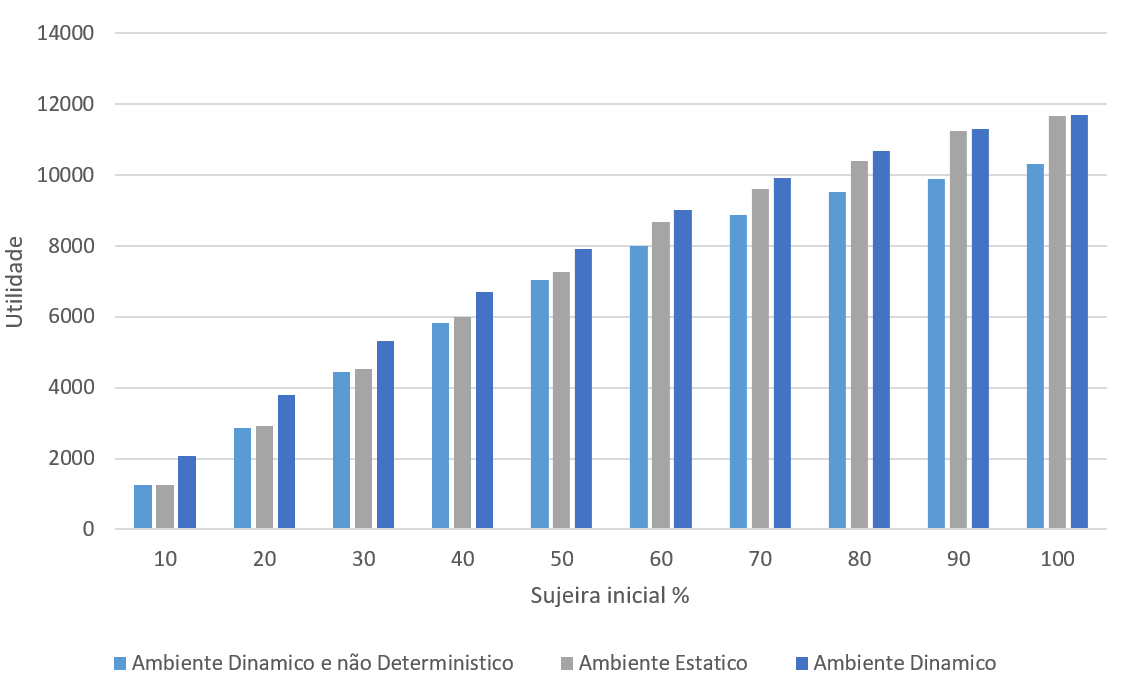
\includegraphics[width=10cm]{figuras/exp2-perf-utilidade.png}
    }{
        \Fonte{Elaborado pelo autor}
    }   
\end{figure}

Na Figura \ref{fig:exp2-perf-utilidade} acima podemos perceber que de todos os cenários observados, o que exibe um melhor desempenho é o cenário associado ao agente determinístico inserido em um ambiente dinâmico.  Isso acontece devido ao fato de a todo instante o ambiente depositar novas sujeiras em \textit{patches} limpos, aumentando o desempenho associado a função $av_1$ e, consequentemente, a utilidade.  O agente não determinístico possui o pior desempenho pois é o único com a desvantagem capaz de afetar a função $av_1$. 

\begin{figure}[h!]
    \centering
    \Caption{\label{fig:exp2-perf-limpeza} Distribuição do objetivo $O_1$ no experimento 2.} 
    \UECEfig{}{
        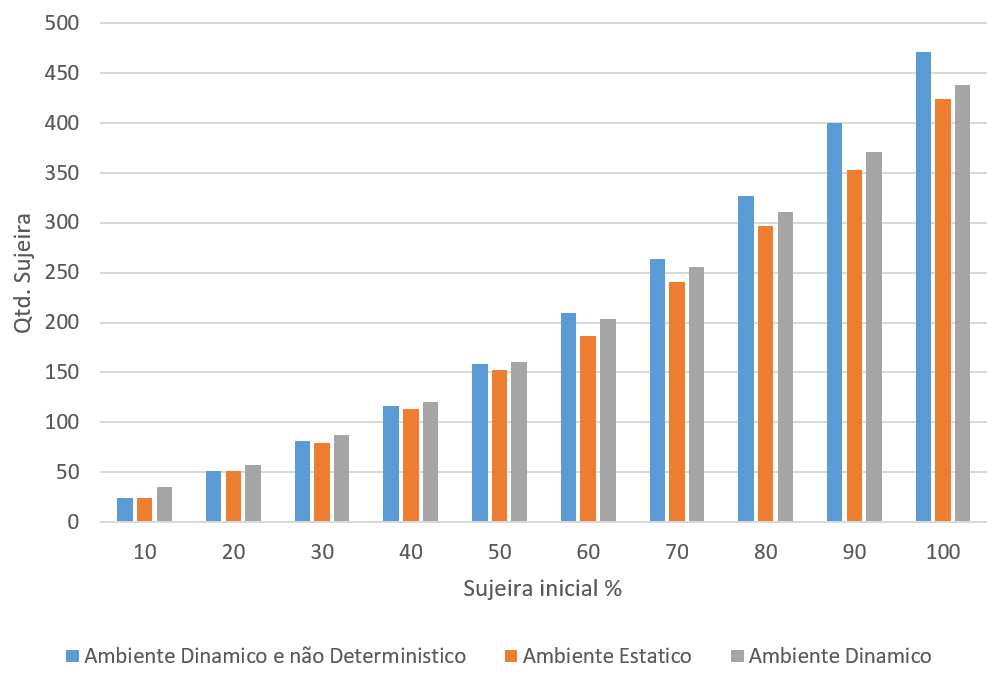
\includegraphics[width=10cm]{figuras/exp2-perf-limpeza.png}
    }{
        \Fonte{Elaborado pelo autor}
    }   
\end{figure}

As medidas associadas a quantidade de sujeira no fim do experimento deixam claro o quanto as falhas nos componentes do agente afetam em seu objetivo. Novamente o agente determinístico em ambiente estático teve um desempenho melhor, como era esperado. Mas o experimento em ambiente dinâmico, que também utiliza um agente determinístico, apresentou uma performance bastante similar. 

\subsection{Sistema \textit{AmI} com um único sistema técnico em um ambiente com pessoas}
\label{sec:exp-user}
No experimento anterior observamos o comportamento do sistema operando com um único agente aspirador em um ambiente vazio e sem circulação de pessoas. No entanto, na aplicação real serão raras as ocasiões em que o agente estará sozinho no ambiente. Para tornar essa simulação um pouco mais condizente com realidade, neste experimento, vamos inserir no modelo do sistema um conjunto de agentes usuários que circulam pelo e ambiente e o modificam, interagindo com os aspiradores de forma indireta.

Cada agente usuário será representado por um único agente inteligente. Eles utilizam uma arquitetura reativa simples, e seu um único objetivo é sair do ambiente, mas sua principal função neste experimento é atrapalhar os agentes aspiradores. Na simulação, cada agente usuário é representado por um círculo azul, como ilustrado na Figura \ref{fig:exp2-5users}. 

\begin{figure}[h!]
    \centering
    \Caption{\label{fig:exp2-5users} Simulação do ambiente com cinco usuarios e um aspirador.} 
    \UECEfig{}{
        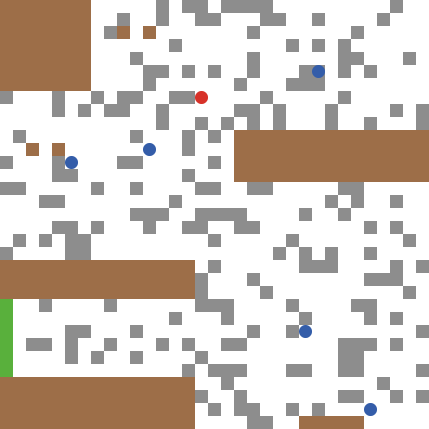
\includegraphics[width=6cm]{figuras/exp2-5users.png}
    }{
        \Fonte{Elaborado pelo autor}
    }   
\end{figure}

Este experimento será realizado no mesmo ambiente de simulação utilizado na seção \ref{sec:exp-dinamico}, ou seja, os agentes estarão inseridos em um ambiente dinâmico, que muda com o passar do tempo. Os aspiradores também deverão manter seus componentes não determinísticos que representam suas falhas. Dessa forma, os usuários serão inseridos em um ambiente dinâmico e não determinístico, mais próximo do que seria em um ambiente real. 

Conforme descrito na segunda seção do Capítulo \ref{cap:abordagem}, a proposta \textbf{P3} na abordagem consiste em uma descrição do sistema \acrshort{ami} por meio de uma organização de programas de agentes racionais, representando o \textit{software} e o \textit{hardware} componentes do sistema técnico, mas também as pessoas usuárias deste sistema. No que diz respeito ao modelo \acrshort{fec} da organização simulada nos experimentos anteriores, os modelos $F$, $E$ e $C$ neste experimento foram estendidos para acomodar as pessoas no sistema \acrshort{ami}. As subseções a seguir especificam o que foi estendido. 

\subsubsection{Modelo F}

Esta seção ilustra as alterações nos componentes do modelo $F$ da organização relacionados ao programa $AgSoftware$ no papel $Controller$ empregado nos dois experimentos anteriores. Apesar da presença de pessoas no ambiente, também representadas por programas de agentes na organização, a seção não dá ênfase às alterações nos componentes do modelo $F$ associados aos programas no papel de usuários, visto que os experimentos estão registrando o desempenho do programa no papel $Controller$. Entretanto, o mesmo tipo de especificação pode ser feito para os programas representando pessoas.

A Figura \ref{fig:arq-agent-amb} ilustra uma interação do sistema técnico ($AgentAmI$ = $AgSoftware$, \textit{hardware} formado por um sensor e um atuador) com o ambiente em um instante $k$. Diferente do primeiro experimento, considerando que existem pessoas no ambiente, em qualquer instante $k$ o sensor do aspirador percebe ($s^{*k}$) uma grade de $32 \times 32$ \textit{patches}, os quais podem ser do tipo limpo, sujo, obstáculo ou pessoa. Assim, a primeira alteração no modelo $F$ está na descrição dos estados do ambiente do aspirador de pó:

\begin{itemize}
    \item $S = \{s^1, s^2, \ldots\}$ --	Estados do ambiente – em qualquer instante $k$ o agente $AgSoftware$ recebe o estado $s^k$ consistindo de uma grade de $3\times3$ \textit{patches}, contida no ambiente definido pelo cenário, que mostra as características dos \textit{patches} (branco, cinza e marrom) e quais agentes estão sobre eles (usuário e aspirador);
    
    \item $\textrm{ação} : S^*  \rightarrow A$ -- Comportamento – função para seleção de ações em $A$ adequadas aos estados em $S$, ou seja: o aspirador deve limpar \textit{patches} cinza, mudar para um \textit{patch} vizinho que seja cinza se estiver em um \textit{patch} branco, e deve mudar de direção se estiver em frente a um usuário;
    
\end{itemize}

A inserção de usuários no sistema permite que seja observada uma outra característica importante no seu desempenho. Para isso, devemos atualizar o objetivo original ($O_O$). Agora, além dos objetivos anteriores, manter o ambiente limpo e economizar energia, o agente aspirador deve também priorizar o bem estar dos usuários, evitando incomodá-los enquanto caminham pelo ambiente. Dessa forma, o objetivo original passa a ser composto por três vetores, ilustrados na tabela \ref{tab:objetivo-exp3}.

\begin{table}[h!]   
    \centering
    \Caption{\label{tab:objetivo-exp3} Objetivos próximos do terceiro experimento.}
    \UECEtab{}{
        \begin{tabular}{cccc}
            \toprule
                Objetivo &  Descrição   &   Função Objetivo & Recompensa \\
                \midrule \midrule
                $O_1$  & Manter o ambiente limpo & $f_1(H(Cenarios))$ & $av_1(Ep^k(h(Cenario_i)))$ \\
                $O_2$  & Manter energia na bateria & $f_2(H(Cenarios))$ & $av_2(Ep^k(h(Cenario_i)))$ \\
                $O_3$  & Evitar colisões com usuários & $f_3(H(Cenarios))$ & $av_3(Ep^k(h(Cenario_i)))$ \\
            \bottomrule
        \end{tabular}
    }{
    \Fonte{Elaborado pelo autor}
}
\end{table}

As funções escalares $av_1$ e $av_2$, definidas no experimento anterior não serão afetadas diretamente com a inserção dos agentes usuários. Mas agora precisamos definir uma função que associe o objetivo $O_3$ a um valor escalar, representando o desempenho do agente neste objetivo. A função $av_3$ é descrita em função do conjunto de episódios $Ep(s, a) \in S\times A$, onde $s \in S$ e $a \in A$. A definição dessa função é mostrada na equação abaixo. 

\[
Av_3(Ep((s^k, a^k)) =
\begin{cases}
  15 & \text{se $s^k$ = frente norte e azul e $a^k$ = norte,}\\
  15 & \text{se $s^k$ = frente sul e azul e $a^k$ = sul,}\\
  15 & \text{se $s^k$ = frente leste e azul e $a^k$ = leste,}\\
  15 & \text{se $s^k$ = frente oeste e azul e $a^k$ = oeste,}\\
  0 & \text{se $s^k$ = frente X e não azul e $a^k$ = Y,}\\
\end{cases}
\]
 tal que $X, Y \in \{ norte, sul, leste, oeste\}$ 

A função descrita acima associa os episódios em que o agente aspirador percebe usuários posicionados a sua frente e seleciona a ação de colidir. Essa ação representa a tentativa do agente aspirador de se mover em direção a um \textit{patch} já ocupado por um usuário. Dessa forma, em um conjunto formado por N cenários, onde cada cenários possui uma história de M episódios, temos que a função associada a $O_3$ é:

\begin{equation}
    f_3(H(Cenarios)) = \frac{1}{N}\sum_{k=1}^{N}Av_3(h(Cenario_i))
\end{equation}
, onde:
\begin{equation}
    Av_3(h(Cenario_i)) = \sum_{k=1}^{M}(Ep(s^k, a^k)
\end{equation}

Para finalizar o modelo F, a função utilidade do agente aspirador deve ser atualizada para medir os valores observados pela função $f_3$. Neste experimento consideramos que o objetivo $O_3$ tem um valor de importância maior que os outros objetivos. Portanto, a função utilidade do objetivo original do sistema será:
\begin{equation}
    Utilidade(f (H(Cenarios)))= f_1 (H(Cenarios)) + f_2 (H(Cenarios)) - 2 \times f_3 (H(Cenarios))
\end{equation}

Com essa atualização na função Utilidade, é possível observar o desempenho do sistema em situações onde o agente em um ambiente com usuários. Quanto mais usuários no ambiente, maiores serão as chances do aspirador se chocar com algum usuário, diminuindo o valor de utilidade e, portanto, seu desempenho. 

\subsubsection{Modelo E}

Como o usuário não faz parte do sistema técnico da aplicação, ele deve ser representado por um único agente. Isso significa que não existirão intermediários entre ele e o ambiente, logo suas percepções e ações dependem apenas de seus próprios sensores e atuadores. O programa de agente que interpreta o usuário na aplicação é chamado $AgUser$.

A definição da organização sistema elaborada no primeiro deve ser atualizada para que contemple também o agente usuário. Associando o programa de agente usuários aos seus respectivos papéis e ainda definindo suas relações com os outros agentes definidos previamente. 

\begin{itemize}
    \item Agents --	$\{AgHardware_1, AgHardware_2, AgSoftware, AgUser \}$ – conjunto de programas $AgentAmI$ na organização ($N_A = 4$).
    
    \item Roles	-- $\{Device, Controller, User\}$ – conjunto de papéis ($N_R = 3$) que podem ser atribuídos aos programas de agentes $AgentAmI$.
    
    \begin{itemize}
        \item $AgentAmIUser$ -- $\{AgUser_1, \ldots, AgUser_N\}$ – conjunto de programas no papel $User$;
    \end{itemize}
    
    \item $Bond_{knowledge}(AgentAmISoftware, AgentAmIUser)$ -- $\{$($AgSoftware$, $AgUser_1$), $\ldots$, ($AgSoftware$, $AgUser_M$)$\}$ – programa AgSoftware (papel $Controller$) têm o conhecimento da existência dos programas $AgUser_1, \ldots, AgUser_M$ (papel $User$), tal que $0 \leq M \leq N$;
    
    \item Groups -- \{$AgHardware_1$, $AgHardware_2$, $AgSoftware$, $AgPessoa_1$, $\ldots$, $AgPessoa_N$\} – família de um ($N_G = 1$) conjunto de programas de agentes exercendo seus papéis na organização.
\end{itemize}

As definições acima atualizam os conjuntos definidos nos experimentos anteriores. Os grupos omitidos não sofreram alterações. A última parte do modelo $E$ define os relacionamento de comunicação entre os agente. Porém, como o agente usuário não interage diretamente com nenhum agente do sistema técnico, não há necessidade de estabelecer um processo de comunicação entre eles. 

\subsubsection{Modelo C}

O modelo $C$ também deve ser atualizado neste experimento para descrever o comportamento do agente usuário e adequar o desempenho do agente aspirador aos novos estímulos. O agente usuário, por não precisar apresentar um comportamento complexo, é representado por um agente reativo simples, assim como os agentes $AgHardware_1$ e $AgHardware_2$ descritos no experimento anterior.  A Figura \ref{fig:exp3-modelC} abaixo mostra um esboço do agente usuário interagindo com o ambiente juntamente com os agentes definidos previamente.

\begin{figure}[h!]
    \centering
    \Caption{\label{fig:exp3-modelC} Esqueletos dos agentes definidos no terceiro experimento.} 
    \UECEfig{}{
        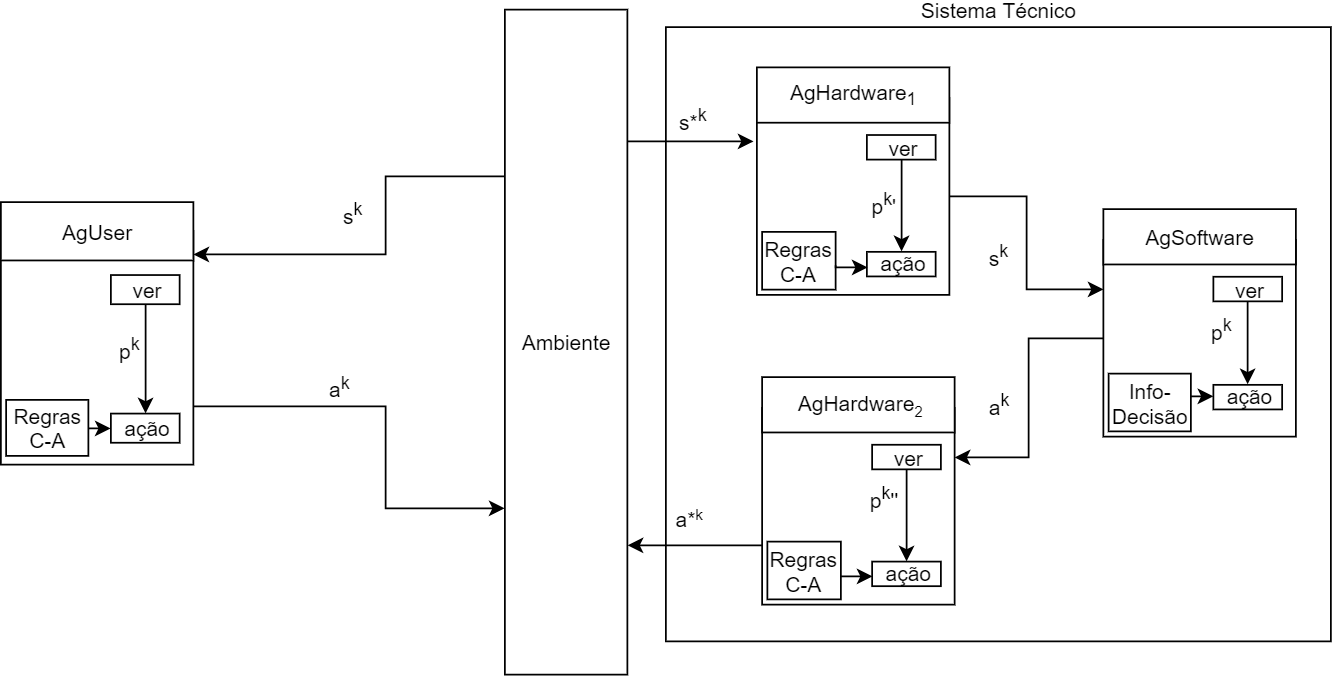
\includegraphics[width=10cm]{figuras/exp3-modelC.png}
    }{
        \Fonte{Elaborado pelo autor}
    }   
\end{figure}

O agente usuário enxerga o conjunto de estados do ambiente $s^k$ e utiliza sua função ver para extrair informação desse conjunto, formando sua percepção $p^k$. Utilizando suas regras C-A, o usuário informa ao ambiente qual foi a ação selecionada. O algoritmo \ref{alg:exp3-behaviour} abaixo apresenta o conjunto de regras condição-ação do agente usuário. 

\begin{algorithm}[h!]
    %\SetSpacedAlgorithm
    \caption{\label{alg:exp3-behaviour} Conjunto de regras condição-ação do programa $AgUser$.}
    %\Entrada{$p^k$ em S}
    %\Saida{$a^k$ em A}
    função ação ($p^{k\prime\prime}$ em P) retorna $a^{*k}$ em A\\
    \Inicio{
        \ldots\\
        \textbf{se} $p^{k}$ = cinza \textbf{então} $a^{*k}$ = move-random\;
        \textbf{se} $p^{k}$ = branco \textbf{então} $a^{*k}$ = throw-dirt\;
        \textbf{se} $p^{k}$ = verde \textbf{então} $a^{*k}$ = get-out\;
        \textbf{se} $p^{k}$ = marrom \textbf{então} $a^{*k}$ = change-dir\;
        \ldots\\
    }
\end{algorithm}

Sempre que o agente usuário fica sobre um \textit{patch} sujo, ele se move para um \textit{patch} vizinho aleatório. Se o usuário estiver sobre um \textit{patch} limpo a função \textit{throw-dirt} é acionada, fazendo com que o \textit{patch} se torne sujo com uma certa probabilidade. Nos experimentos realizados neste trabalho, a função \textit{throw-dirt} tem uma probabilidade de 5\% de sujar locais que o agente o usuário passa. A função \textit{get-out} é acionada sempre que o agente usuário encontrar a saída, representada por um conjunto de \textit{patches} verdes, quando executada o usuário sai do ambiente. 

Com relação ao aspirador, para que ele continue de acordo com o que foi definido no modelo $F$, é preciso atualizar suas regras condição-ação obedecendo aos objetivos adicionados. O objetivo próximo $O_3$, definido no modelo de função deste experimento, estabelece que o agente aspirador deve evitar incomodar os usuários prevenindo qualquer colisão com eles. Para isso, adicionamos a seguinte regra na base do agente AgSoftware:

\begin{algorithm}[h!]
    %\SetSpacedAlgorithm
    \caption{\label{alg:exp3-behaviour-asp} Nova regra do agente AgSoftware.}
    %\Entrada{$p^k$ em S}
    %\Saida{$a^k$ em A}
    função ação ($p^{k\prime\prime}$ em P) retorna $a^{*k}$ em A\\
    \Inicio{
        \ldots\\
        \textbf{se} user-close($p^{k}$) \textbf{então} $a^{*k}$ = move-away\;
        \ldots\\
    }
\end{algorithm}

A função \textit{user-close}, verifica o conjunto de percepções do agente aspirador buscando um agente usuário. Se for identificado que existe um usuário em uma posição dentro do raio de percepção do agente a função \textit{move-away} é acionada. Essa função usa a posição do usuário e a direção para a qual ele está apontando para determinar o caminho por onde ele deverá percorrer. Se a posição do aspirador estiver neste caminho, o aspirador deve girar noventa graus em relação ao usuário e se mover para o \textit{patch} vizinho.

Tendo em vista que os agentes usuários e os aspiradores não se comunicam diretamente, não é necessário alterar o comportamento de comunicação, definido anteriormente, para o agente aspirador. Na seção a seguir apresentamos os objetos emergentes obtidos na simulação criada a partir do modelo \acrshort{fec} apresentado. 

\subsubsection{Objetos Emergentes}

Diferente do experimento anterior, a quantidade inicial de sujeira no ambiente será mantida fixa em 25\% em todas as execuções. Nesta terceira prática, vamos observar o desempenho do agente AgSoftware no ambiente à medida que novos usuários são inseridos. Serão observados quinze cenários diferentes, no primeiro serão inseridos cinco usuários no ambiente de simulação, e a  cada cenário seguinte serão inseridos mais cinco, totalizando 75 usuários no ultimo experimento.

\begin{figure}[h!]
    \centering
    \Caption{\label{fig:exp3-sim-exec} Objetos emergentes em uma execução da simulação.} 
    \UECEfig{}{
        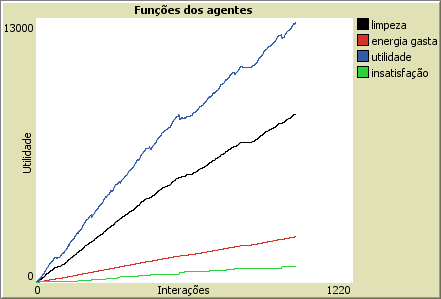
\includegraphics[width=8cm]{figuras/exp3-sim-exec.png}
    }{
        \Fonte{Elaborado pelo autor}
    }   
\end{figure}

A Figura \ref{fig:exp3-sim-exec} mostra as distribuições de cada um dos objetivos próximos do sistema durante a execução de um cenário que contem vinte usuários. A insatisfação, apresentada na cor verde, indica o desempenho do agente relacionado ao objetivo próximo $O_3$.  A Figura \ref{fig:exp3-perf-utilidade} abaixo apresenta um histograma da utilidade do aspirador durante os quinze cenários do experimento. 

\clearpage
\begin{figure}[h!]
    \centering
    \Caption{\label{fig:exp3-perf-utilidade} Utilidade do terceiro experimento.} 
    \UECEfig{}{
        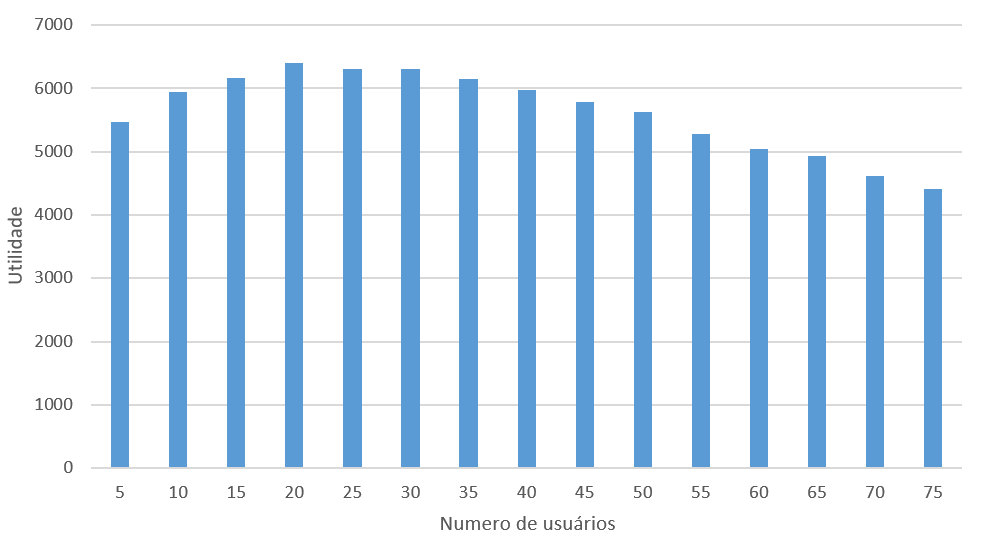
\includegraphics[width=10cm]{figuras/exp3-perf-utilidade.png}
    }{
        \Fonte{Elaborado pelo autor}
    }   
\end{figure}

Como podemos observar na Figura \ref{fig:exp3-perf-utilidade}, o valor da utilidade do agente aspirador, em um primeiro momento, cresce juntamente com o número de usuários no ambiente. Porém, do quinto cenário em diante esse valor passa a decrescer. Esse crescimento inicial é atribuído à propriedade do usuário de gerar novas sujeiras no ambiente, facilitando a busca do aspirador e consequentemente alimentando o objetivo próximo de manter o ambiente limpo ($O_1$). Mas a medida que o número de usuários cresce nos cenários seguintes, a utilidade passa a decrescer devido as penalidades impostas pelo novo objetivo próximo $O_3$, inserido nesse experimento. 

\begin{figure}[h!]
    \centering
    \Caption{\label{fig:exp3-perf-limpeza} Desempenho de limpeza no terceiro experimento.} 
    \UECEfig{}{
        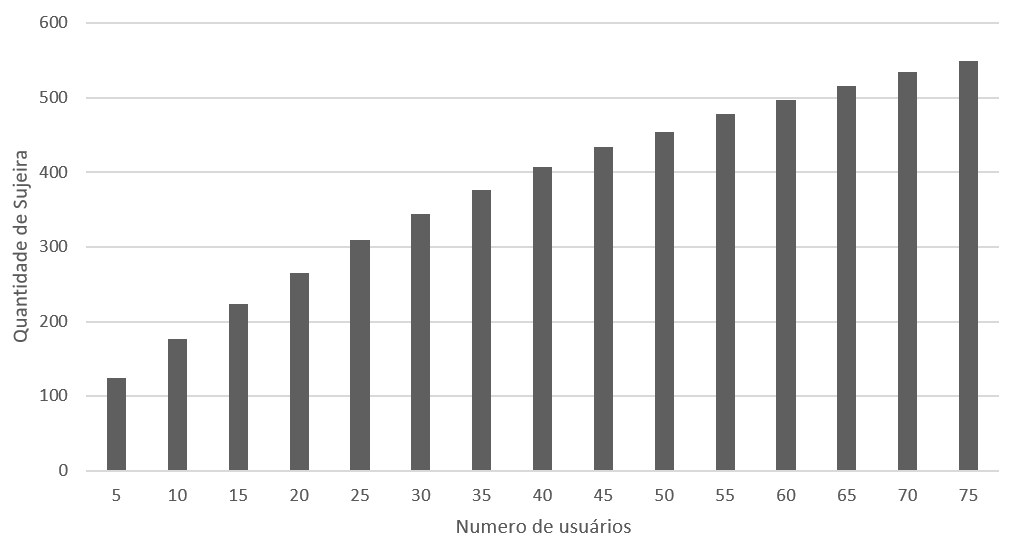
\includegraphics[width=10cm]{figuras/exp3-perf-limpeza.png}
    }{
        \Fonte{Elaborado pelo autor}
    }   
\end{figure}

A Figura \ref{fig:exp3-perf-limpeza} acima apresenta a variação de sujeira ao fim de cada um dos cenários.  É fácil perceber que quanto mais usuários no ambiente maior será a quantidade de sujeira inserida nele. Isso mostra que um único agente aspirador não é suficiente para manter o ambiente limpo quando grandes quantidades de pessoas circulam por ele.

\subsection{Sistema \textit{AmI} com múltiplos aspiradores}
\label{sec:multi-asp}
No experimento anterior, inserimos um novo agente usuário, representando as pessoas que utilizarão o sistema \acrshort{ami}, em um ambiente dinâmico interagindo com um único agente aspirador não determinístico. Neste quarto experimento, vamos inserir outros aspiradores no ambiente e observar o desempenho do sistema em satisfazer seu objetivo original. 

O aspirador é representado por um conjunto de agentes que simulam o comportamento do aspirador de pó no ambiente. Cada aspirador é composto por dois agentes do tipo $AgHardware$ e um do tipo $AgSoftware$, como mostrado nos experimentos anteriores. As extensões inseridas no modelo \acrshort{fec} são explicadas a seguir.

\subsubsection{Modelo F}

Diferente do experimento anterior, que considera a existência de pessoas no ambiente, em qualquer instante $k$ o sensor do aspirador percebe ($s^{*k}$) uma grade de $32 \times 32$ \textit{patches}, os quais podem ser do tipo limpo, sujo, obstáculo, pessoa ou aspirador. Assim, a única alteração no modelo $F$ está na descrição dos estados do ambiente do aspirador de pó: 

\begin{itemize}
    \item $S = \{s^1, s^2, \ldots\}$ -- Estados do ambiente – em qualquer instante $k$ o sensor do aspirador disponibiliza um estado $s^k$ consistindo de uma grade menor, contida na grade $32 \times 32$ \textit{patches} que representa o local, de tamanho $3 \times 3$ \textit{patches}, ou seja, o conjunto de estados do ambiente é formado por todas as grades desse tamanho, em que cada \textit{patch} pode representar uma parte limpa (branco) ou suja (cinza) do local, ou a presença de um obstáculo (marrom), de uma pessoa (azul), ou de um aspirador (vermelho).
\end{itemize}

Apesar da presença de outros aspiradores, o objetivo original do sistema não foi modificado, mas é importante explicitar que outros objetivos poderiam ser adicionados. Poderíamos considerar como um outros objetivos próximos evitar colisões entre os próprios aspiradores, ou a cooperação entre eles. Porém, como o objetivo deste trabalho é apenas definir um modelo de criação de sistemas \acrshort{ami}, foi optado um caminho mais simples, mantendo os objetivos definidos anteriormente. 

\subsubsection{Modelo E}

A Figura \ref{fig:exp4-org-modelE} consiste em uma organização de programas de agentes racionais representando o sistema \acrshort{ami} formado por $M$ aspiradores de pó independentes. Cada programa $AgSoftware_i$ processa as informações perceptivas oriundas do processamento de seu programa $AgHardware_{1i}$, seleciona ações que evitem colisões com cada um dos $N$ programas representando pessoas, e envia estas ações para o seu programa $AgHardware_{2i}$, o qual as executa no ambiente.

\begin{figure}[h!]
    \centering
    \Caption{\label{fig:exp4-org-modelE} Organização de agentes no experimento quatro.} 
    \UECEfig{}{
        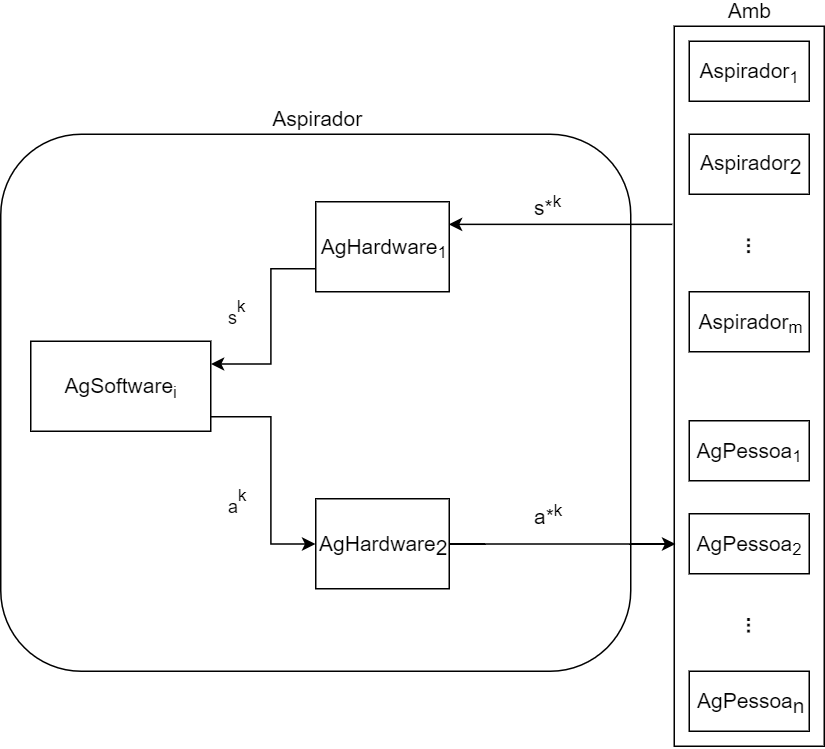
\includegraphics[width=8cm]{figuras/asp-exp4.png}
    }{
        \Fonte{Elaborado pelo autor}
    }   
\end{figure}

Quanto ao modelo E associado à figura, é necessário estender o conjunto de programas de agentes e de papéis que os programas podem assumir na organização, e de relações entre programas especificadas no último experimento, ou seja:

\begin{itemize}
    \item Agents -- \{$AgHardware_{11}$, $AgHardware_{21}$, $AgSoftware_1$, \ldots, $AgHardware_{1M}$, $AgHardware_{2M}$, $AgSoftware_M$, $AgPessoa_1$, \ldots, $AgPessoa_N$\} – conjunto $N_A = N + 3 \times M$ programas $AgentAmI$ na organização.
    
    \item AgentAmIDevice	\{$AgHardware_{11}$, $AgHardware_{21}$,  \ldots, $AgHardware_{1M}$, $AgHardware_{2M}$\} – conjunto de programas no papel \textit{Device};
    
    \item AgentAmIController	\{$AgSoftware_1$, \ldots, $AgSoftware_M$\} – conjunto de programas no papel \textit{Controller}.
    
    \item Bond	\{$Bond_{knowledge}$($AgentAmIDevice$, $AgentAmIController$),\\
            $Bond_{knowledge}$($AgentAmIControlle$r, $AgentAmIDevice$),\\
            $Bond_{\textrm{Coordenação}}$($AgentAmIDevice$, $AgentAmIController$),\\
            $Bond_{\textrm{Coordenação}}$($AgentAmIController$, $AgentAmIDevice$),\\
            $Bond_{knowledge}$($AgentAmIController$, $AgentAmIUser$),\\
            $Bond_{knowledge}$($AgentAmIController$, $AgentAmIController$)\} – família de seis relações entre os programas nos conjuntos $AgentAmIDevice$, $AgentAmIController$ e $AgentAmIUser$ tal que:
    
    \begin{itemize}
        \item $Bond_{knowledge}$($AgentAmIController$, $AgentAmIController$) --	\{($AgSoftware_1$, $AgSoftware_2$), \ldots , ($AgSoftware_1$, $AgSoftware_M$), \ldots, ($AgSoftware_M$, $AgSoftware_1$), \ldots, ($AgSoftware_M$, $AgSoftware_{M-1}$)\} – programa $AgSoftware_i$ (papel $Controller$) têm o conhecimento da existência dos programas $AgSoftware_1$, \ldots, $AgPessoa_N$ (papel $User$), tal que $0 \leq i \leq M$;
    \end{itemize}
    
    \item Groups -- \{$AgHardware_{11}$, $AgHardware_{21}$, $AgSoftware_1$, \ldots, $AgHardware_{1M}$, $AgHardware_{21}$, $AgSoftware_M$, $AgPessoa_1$, \ldots, $AgPessoa_N$\} – família de um ($N_G = 1$) conjunto de programas de agentes exercendo seus papéis na organização.
    
\end{itemize}

As informações apresentadas no modelo $E$ do último experimento que não são mencionadas no quadro acima não sofreram alterações com a adição  de outros aspiradores no ambiente. Apesar de cada programa $AgSoftware_i$ no papel $Controller$ poder conhecer um número $M-1$ de programas no papel $Controller$, não existe troca de mensagens entre eles. Dessa forma, a matriz sociométrica do primeiro experimento também não sofre alteração. 

\subsubsection{Modelo C}
Apesar dos aspiradores não trocarem mensagens entre si, o modelo comportamental descrito anteriormente foi estendido. O subsistema de tomada de decisão do programa AgSoftware sofreu alteração visando incorporar as percepções sobre os programas aspiradores (\textit{patches} em vermelho na simulação NetLogo), ou seja, pela presença de novas regras no conjunto. Mais especificamente, estas regras possibilitam que um aspirador evite colisões com outros aspiradores, mudando a direção de seu movimento sempre que perceber que está diante de outro aspirador no ambiente.

\subsubsection{Objetos Emergentes}

Para observar o comportamento do sistema neste experimento, analisamos três configurações do ambiente variando a quantidade de agentes aspiradores e de agentes usuários. Na primeira configuração fixamos a quantidade de aspiradores em três e variamos a quantidade de usuários da mesma forma que o experimento anterior. Na segunda dobramos a quantidade de agentes aspiradores, sendo seis agora.  E na terceira passam a circular no ambiente um total de doze agentes aspiradores. A Figura \ref{fig:exp4-perf-utilidade} abaixo mostra as distribuições obtidas observando a média da utilidade dos agentes. 

\begin{figure}[h!]
    \centering
    \Caption{\label{fig:exp4-perf-utilidade} Variação da utilidade no quarto experimento.} 
    \UECEfig{}{
        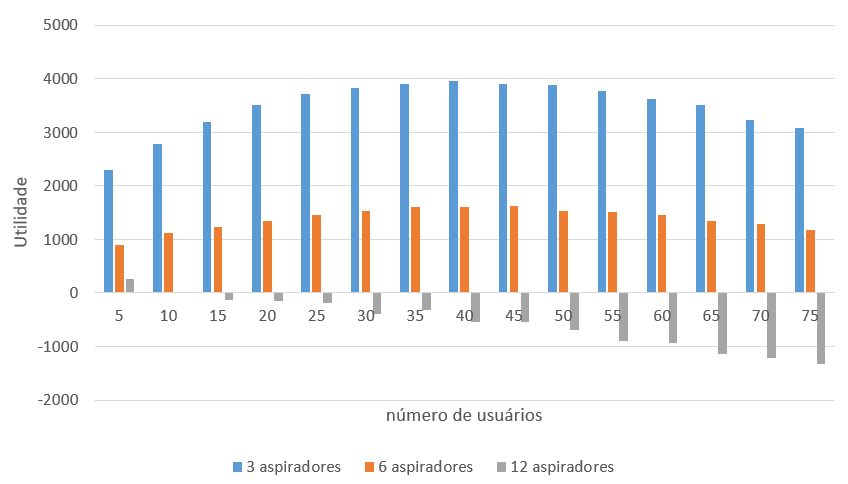
\includegraphics[width=10cm]{figuras/exp4-perf-utilidade.png}
    }{
        \Fonte{Elaborado pelo autor}
    }   
\end{figure}

Como o valor observado é a média das utilidades de cada um dos aspiradores, era esperado que os valores de utilidade decrescessem muito quando comparados aos experimentos anteriores. Um outro fator que também diminui a performance dos agentes neste experimento é quantidade de usuários. A medida que o número de pessoas no ambiente cresce a possibilidade dos aspiradores colidirem com eles também sobe, e como o peso associado ao objetivo próximo $O_3$ é maior que os outros, isso acaba causando uma grande queda nas medidas do $O_O$.

\begin{figure}[h!]
    \centering
    \Caption{\label{fig:exp4-perf-limpeza} Variação da limpeza no ambiente no quarto experimento.} 
    \UECEfig{}{
        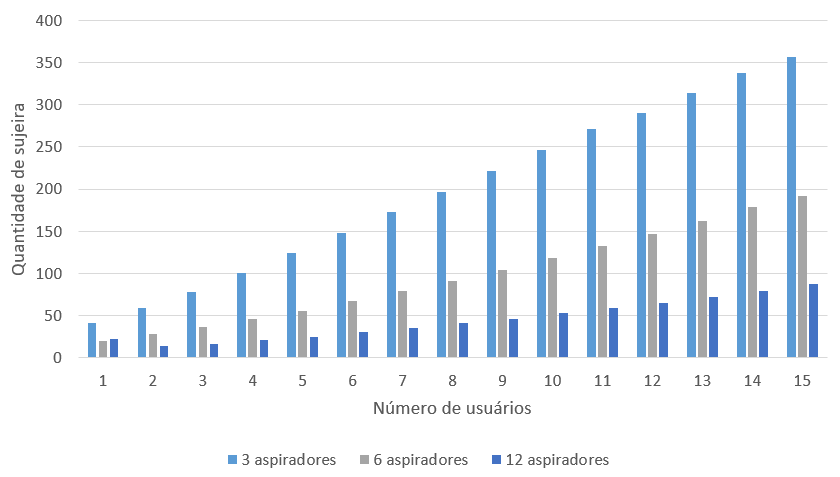
\includegraphics[width=10cm]{figuras/exp4-perf-limpeza.png}
    }{
        \Fonte{Elaborado pelo autor}
    }   
\end{figure}

Com relação a sujeira no ambiente, a Figura \ref{fig:exp4-perf-limpeza} acima deixa bem claro que a quantidade de aspiradores é uma propriedade muito importante para a limpeza do ambiente. Porém, como vimos na distribuição exibida pela Figura \ref{fig:exp4-perf-utilidade}, é necessário que exista uma mudança de estratégia para que o desempenho do sistema não seja afetado. 

\subsection{Sistema \textit{AmI} com Agentes Coordenadores}
\label{sec:exp-coord}

No experimento anterior observamos o desempenho de um sistema \acrshort{ami}, composto por diversos agentes aspiradores, interagindo com múltiplos usuários em um ambiente. Apesar da grande quantidade de aspiradores apresentar bons resultados, em relação a limpeza do ambiente, sua utilidade tende a ser muito baixa. 

Esse desempenho é uma consequência direta do comportamento dos aspiradores. Apesar de existir um time de agentes que possuem o mesmo objetivo, não há nenhum tipo de cooperação entre eles. Cada um age como se estivesse sozinho, sem nenhuma comunicação com outros agentes. Além disso, a estratégia utilizada para buscar sujeira no ambiente obriga os aspiradores a se movimentarem continuamente, procurando por \textit{patches} sujos em áreas que já foram completamente limpas. 

Para tentar melhorar o desempenho do sistema, vamos adicionar uma nova entidade que estende o agente aspirador chamada de agente coordenador. Essa entidade será responsável por enviar mensagens a outros aspiradores, informando sobre locais com alta concentração de sujeira ou solicitando que o aspirador entre em modo de descanso.  Ele será representado na simulação por um círculo verde, como apresentado na Figura \ref{fig:exp5-agent-coord}.

\begin{figure}[h!]
    \centering
    \Caption{\label{fig:exp5-agent-coord} Agente coordenador no ambiente simulado.} 
    \UECEfig{}{
        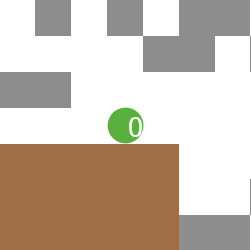
\includegraphics[width=4cm]{figuras/exp5-agent-coord.png}
    }{
        \Fonte{Elaborado pelo autor}
    }   
\end{figure}

Como o coordenador também é um tipo de aspirador, seu modelo de função não será alterado neste momento, porém é necessário alterar seus modelos de estrutura e comportamento. Nas subseções a seguir detalhamos adições necessárias nos modelos \acrshort{fec} para que este agente seja inserido na simulação.  

\subsubsection{Modelo E}

O agente coordenador também é composto por dois agentes do tipo AgHardware, representando seus sensores e atuadores e um do tipo AgSoftware, estruturados da de forma semelhante a apresentada na Figura \ref{fig:exp1-modelC-detail}. A seguir apresentamos as novidades na estrutura deste experimento. 

\begin{itemize}
    \item Agents -- \{$AgHardware_{11}$, $AgHardware_{21}$, $AgSoftware_1$, $AgHardware_{12}$, $AgHardware_{22}$, $AgSoftware_2$, $AgHardware_{13}$, $AgHardware_{23}$, $AgSoftware_3$, \ldots, $AgHardware_{1M}$, \\$AgHardware_{2M}$, $AgSoftware_M$, $AgPessoa_1$, \ldots, $AgPessoa_N$\} – conjunto com $N_A = N + 3 \times (3 + M)$ programas $AgentAmI$ na organização tal que $M \geq 0$, ou seja, existem pelos menos 3 aspiradores no local.

    \item Group --	\{$AgHardware_{11}$, $AgHardware_{21}$, $AgSoftware_1$, \ldots, $AgHardware_{1M}$, $AgHardware_{2M}$, $AgSoftware_M$, $AgPessoa_1$, ..., $AgPessoa_N$\} – família de conjuntos de programas de agentes ($N_G = 1$) exercendo seus papéis na organização.
    
    \item Bond -- \{$Bond_{Authority}(AgentAmIController, AgentAmIController)$\} – Relação de autoridade entre o agente controlador pertencente a um coordenador e um agente controlador pertencente a um aspirador.
    
    \begin{itemize}
        \item \{$Bond_{Authority}(AgentAmIController, AgentAmIController)$\} – \{($AgSoftware_1$, $AgSoftware_4$), ($AgSoftware_1$, $AgSoftware_5$), \ldots, ($AgSoftware_1$, $AgSoftware_M$), ($AgSoftware_2$, $AgSoftware_4$), ($AgSoftware_2$, $AgSoftware_5$), \ldots, ($AgSoftware_2$, $AgSoftware_M$), ($AgSoftware_3$, $AgSoftware_4$), ($AgSoftware_3$, $AgSoftware_5$), \ldots, ($AgSoftware_3$, $AgSoftware_M$)\} – cada  programa $AgSoftware_i$ (papel \textit{Controller}) pode delegar uma ou mais tarefas ao programa $AgSoftware_j$, onde i = \{1, 2, 3\}, e j = \{4, ..., M\};
    \end{itemize}

    \item Communication	-- \{$AgentAmIController$, $AgentAmIController$\} – relação descrevendo quem pode enviar mensagens para quem na organização;

\end{itemize}

O relacionamento de autoridade definido acima permite que um agente no papel \textit{Controller}, que faça parte de um coordenador, seja capaz de delegar tarefas a um outro agente no papel \textit{Controller} em um aspirador. Isso permite que os coordenadores enviem mensagens aos aspiradores contendo informações referentes a tarefas que eles irão executar. Neste experimento foram definidos três agentes, do tipo $AgSoftware$, que pertencem a entidade coordenador. Eles são representados na tabela de relacionamentos acima pelos agentes $AgSoftware_1$, $AgSoftware_2$ e $AgSoftware_3$.

\begin{figure}[h!]
    \centering
    \Caption{\label{fig:estrutura-coordenador} Relações do coordenador com outros agentes no ambiente.} 
    \UECEfig{}{
        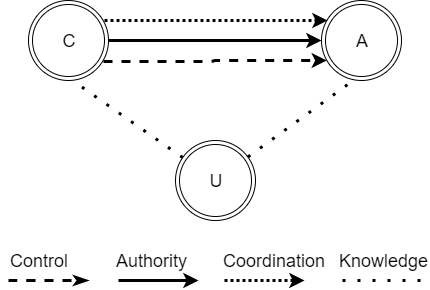
\includegraphics[width=6cm]{figuras/estrutura-coordenador.png}
    }{
        \Fonte{Elaborado pelo autor}
    }   
\end{figure}

A Figura \ref{fig:estrutura-coordenador} ilustra os relacionamentos entre as três entidades do experimento. Assim como o aspirador, o coordenador também tem um relacionamento \textit{knowledge} com o usuário. O que significa que seu relacionamento se limita ao conhecimento da existência um do outro. O relacionamento de autoridade entre o coordenador e o aspirador implica necessariamente na existência dos relacionamentos \textit{control}, \textit{coordination} e \textit{knowledge}.  Ou seja, além de delegar tarefas ao aspirador, este deve manter o coordenador informado sobre suas atividades.  A Figura \ref{fig:exp5-matriz-socio} apresenta a matriz sociométrica que relata a frequência de comunicação entre essas entidades. 

\begin{figure}[h!]
    \centering
    \Caption{\label{fig:exp5-matriz-socio} Matriz de relacionamento entre os agentes do quinto experimento.} 
    \UECEfig{}{
        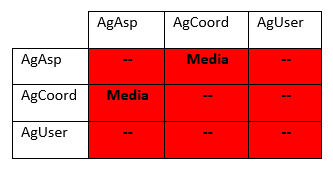
\includegraphics[width=6cm]{figuras/exp5-matriz-socio}
    }{
        \Fonte{Elaborado pelo autor}
    }   
\end{figure}

Apesar de, internamente, os aspiradores e coordenadores serem uma composição de agentes do tipo $AgHardware$ e $AgSoftware$, podemos considerar que todos estão em um mesmo grupo na organização (vermelho). Esses novos relacionamentos inseridos no modelo de estrutura, ainda que simples, levam a grandes mudanças no comportamento dos agentes.  

\subsubsection{Modelo C}

Por ser uma extensão do aspirador, o coordenador também tem os mesmos objetivos definidos no objetivo original do sistema e, portanto, deve se comportar de forma a atingi-los. Mas por ser uma versão melhorada do aspirador, ele possui um conjunto de funções que o tornam mais complexo. A Figura \ref{fig:coordenador} mostra os esqueletos dos programas de agente que representam o coordenador. 

\begin{figure}[h!]
    \centering
    \Caption{\label{fig:coordenador} Esqueletos dos agentes que compõem o coordenador.} 
    \UECEfig{}{
        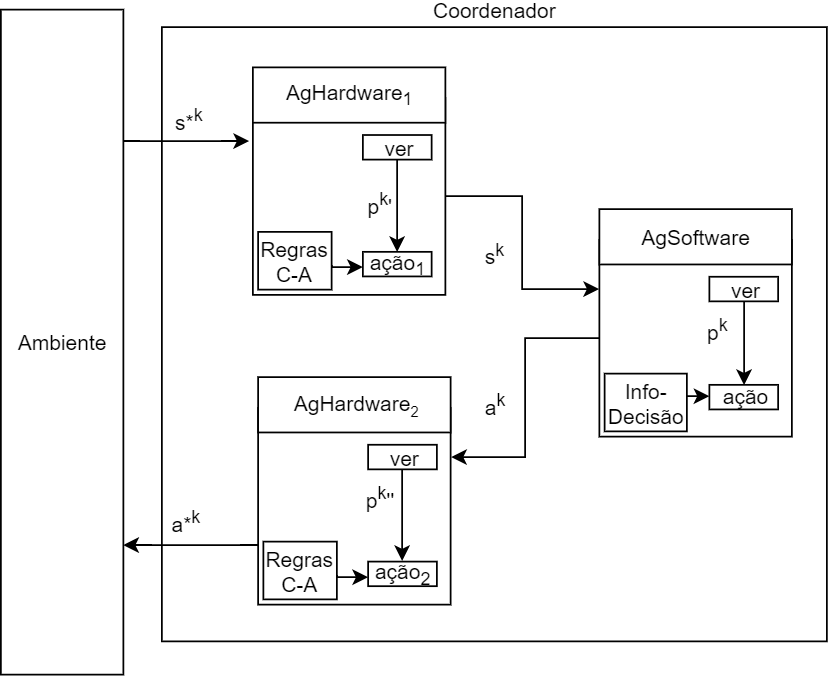
\includegraphics[width=10cm]{figuras/coordenador.png}
    }{
        \Fonte{Elaborado pelo autor}
    }   
\end{figure}

A maior diferença, apresentada na figura acima, entre o coordenador e o aspirador, é que o coordenador possui um AgSoftware do tipo orientado por objetivos. Isso permite que ele tenha um maior poder de decisão, além de possibilitar que sejam armazenadas informações sobre outras entidades do sistema. Abaixo apresentamos uma extensão do modelo F, definido no primeiro experimento, para o agente coordenador.

\begin{itemize}
    \item $P_1 = \{p^{1\prime\prime}, p^{2\prime\prime}, \ldots\}$ -- Percepção do programa $AgHardware_1$ – em qualquer instante $k$ o agente  $AgHardware_1$ ao receber do ambiente entradas perceptivas $s^{*k} \in S$ – estados do ambiente consistindo de uma grade de tamanho $5\times5$ \textit{patches}
    
    \item $\textrm{ação}_1: P_1 \rightarrow S$ -- Subsistema de tomada de decisão de $AgHardware_1$ – função que mapeia percepções $p^{k\prime\prime} \in P_1$ em entradas perceptivas $s^k \in S$ – estados do ambiente consistindo de uma grade de tamanho $5\times5$ \textit{patches} – enviadas para o programa $AgSoftware$.
    
    \item $P = \{p^1, p^2, \ldots\}$ -- Percepção do programa $AgSoftware$ – em qualquer instante $k$ o agente $AgSoftware$ ao receber do programa $AgHardware_1$ as entradas perceptivas $s^k \in S$ – estados do ambiente consistindo de uma grade de tamanho $5\times5$ \textit{patches} – representa estas informações em uma linguagem interna adequada $p^k \in P$.
    
    \item $\textrm{ação}: P \rightarrow A$	-- Subsistema de tomada de decisão de $AgSoftware$ – função que mapeia percepções na linguagem $p^k \in P$ em descrições de ações $a^k \in A$ – enviadas para o programa $AgHardware_2$.
    
\end{itemize}

O sensor do aspirador, definido no modelo de função do primeiro experimento, é capaz de perceber toda sujeira em um raio de três \textit{patches}, já o sensor do coordenador é capaz de sentir sujeira em um raio de até cinco \textit{patches}. Essa nova capacidade permite que o coordenador seja mais eficiente na busca por locais sujos. Ao encontrar sujeira, o coordenador pode enviar suas posições para outros agentes aspiradores no mesmo grupo, ou ir ao local e limpar ele mesmo. 

Além de informar aos aspiradores sobre a localização de sujeiras no ambiente, o coordenador também pode enviar uma série de mensagens para que os aspiradores possam agir de acordo com sua estratégia. Se o aspirador considerar que uma região do ambiente está limpa, ele pode emitir mensagens aos aspiradores próximos para que se movam ou para que entrem em modo de espera, evitando desperdiçar energia. 

\subsubsection{Objetos Emergentes}

As modificações no desempenho do sistema, com relação ao seu objetivo original podem ser observadas na Figura \ref{fig:exp5-perf-utilidade} abaixo.

\begin{figure}[h!]
    \centering
    \Caption{\label{fig:exp5-perf-utilidade} Utilidade do sistema no quinto experimento.} 
    \UECEfig{}{
        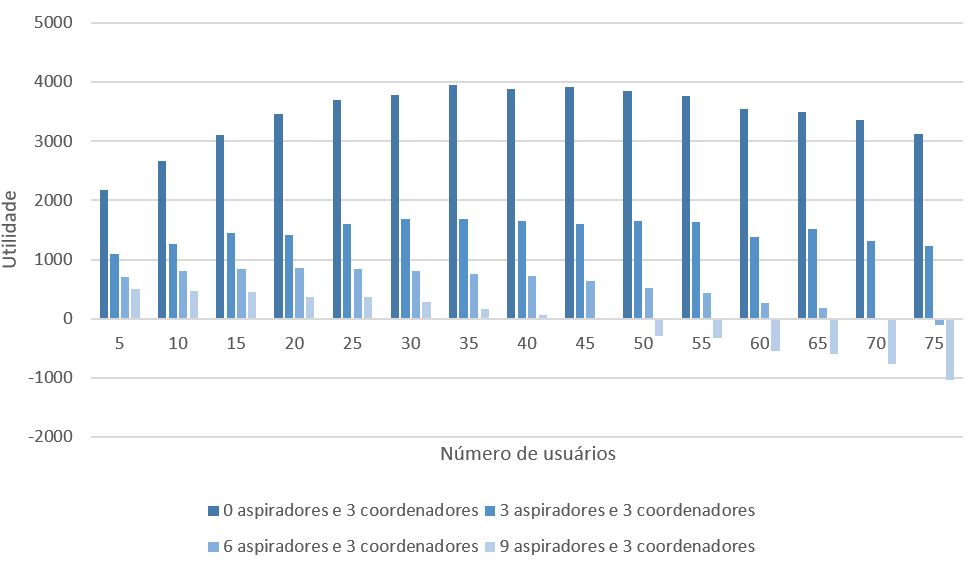
\includegraphics[width=12cm]{figuras/exp5-perf-utilidade}
    }{
        \Fonte{Elaborado pelo autor}
    }   
\end{figure}

A curva de utilidade observada para um primeiro cenário, onde temos apenas 3 agentes coordenadores no ambiente, é similar a curva apresentada no quarto experimento, onde tínhamos três aspiradores simultâneos no ambiente.  O desempenho passa a decrescer com a adição de novos agentes na simulação, porém, apresenta um ganho em relação ao experimento anterior.


\begin{figure}[h!]
    \centering
    \Caption{\label{fig:exp5-perf-limpeza} Limpeza do sistema no quinto experimento.} 
    \UECEfig{}{
        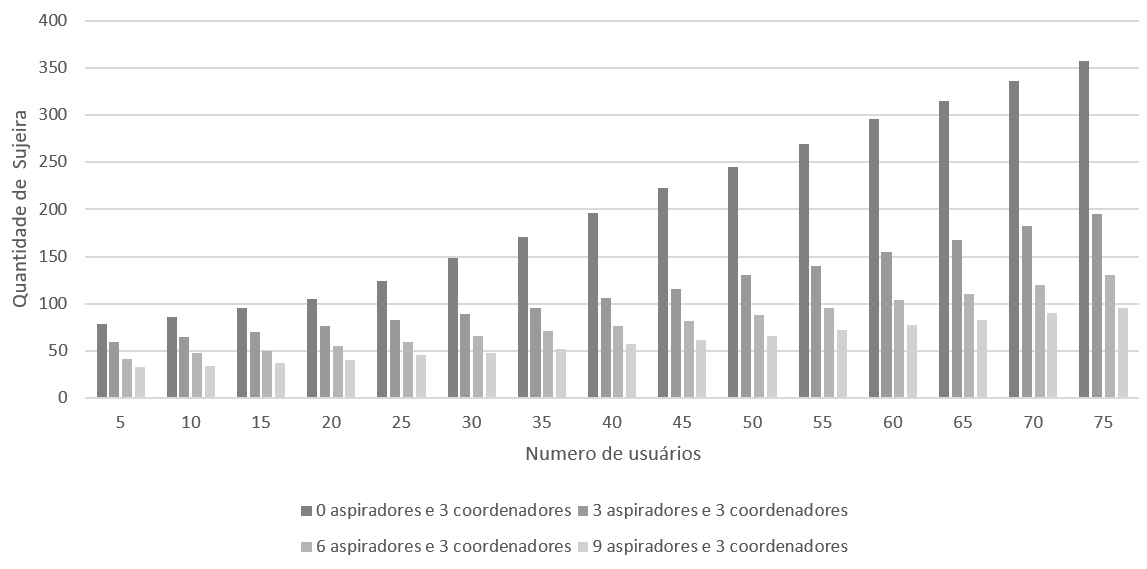
\includegraphics[width=12cm]{figuras/exp5-perf-limpeza}
    }{
        \Fonte{Elaborado pelo autor}
    }   
\end{figure}

Com relação a sujeira do ambiente, não é possível visualizar uma diferença significativa entre a abordagem utilizada no experimento anterior e a atual. Parte disso pode ser explicado pela nova estratégia utilizada, que permite ao coordenador enviar sinais de parada aos demais aspiradores, forçando eles a economizar energia mas impedindo que busquem por sujeira.


\subsection{Sistema \textit{Ami} dividido em Grupos}
\label{sec:grupo}

Para tentar melhorar mais um pouco os valores de utilidade do sistema, neste experimento vamos modificar o modelo de estrutura da organização, dividindo os agentes em três grupos responsáveis por áreas diferentes do ambiente. O objetivo é espalhar melhor os aspiradores e os coordenadores, diminuindo sua necessidade de locomoção e maximizando sua área de cobertura. A Figura \ref{fig:exp6-ambiente} abaixo exemplifica como o ambiente será dividido. 

\begin{figure}[h!]
    \centering
    \Caption{\label{fig:exp6-ambiente} Divisão do ambiente no sexto experimento.} 
    \UECEfig{}{
        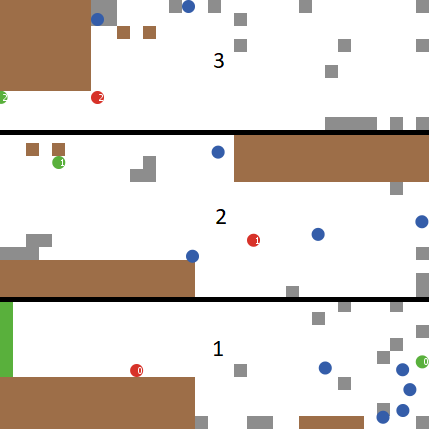
\includegraphics[width=6cm]{figuras/exp6-ambiente.png}
    }{
        \Fonte{Elaborado pelo autor}
    }   
\end{figure}

O ambiente da simulação será dividido em três zonas onde apenas os usuários são livres para circular entre elas. Cada zona terá um agente coordenador responsável, e cada aspirador atuará em uma dessas zonas. Tanto o coordenador quanto o aspirador podem circular apenas por suas zonas. 

Neste experimento, só foi necessário estender o modelo FEC da organização simulada nos experimentos anteriores nas suas dimensões estrutural (E) e comportamental (C), pois não surgiram novas entidades no ambiente, nem novos objetivos próximos. O modelo E foi alterado para acomodar o esquema de divisão em subgrupos. Já o modelo C foi alterado para acomodar os agentes coordenadores.

\subsubsection{Modelo E}

Para que o sistema seja capaz de se dividir no ambiente, conforme mostrado na Figura 54, é necessário estender o modelo de estrutura do conjunto de programas de agentes e de papéis que os programas podem assumir na organização, além das relações entre programas inseridas no último experimento. Mais especificamente, para o caso de três coordenadores conduzindo diferentes subgrupos de aspirador, alocados em zonas distintas do ambiente, onde cada subgrupo contém pelo menos o aspirador de pó coordenador, vale o seguinte modelo estrutural estendido:

\begin{itemize}
    \item Agents -- \{$AgHardware_{11}$, $AgHardware_{21}$, $AgSoftware_1$, $AgHardware_{12}$, $AgHardware_{22}$, $AgSoftware_2$, $AgHardware_{13}$, $AgHardware_{23}$, $AgSoftware_3$, \ldots, $AgHardware_{1M}$, \\$AgHardware_{2M}$, $AgSoftware_M$, $AgPessoa_1$, \ldots, $AgPessoa_N$\} – conjunto com $N_A = N + 3 \times (3 + M)$ programas $AgentAmI$ na organização tal que $M \geq 0$, ou seja, existem pelos menos 3 aspiradores no local, cada um em uma das três zonas e N pessoas espalhadas nas três zonas.

    \item Groups -- \{\{$AgHardware_{11}$, $AgHardware_{21}$, $AgSoftware_1$, \ldots, $AgHardware_{1Ma}$, 
    $AgHardware_{2Ma}$, $AgSoftware_{Ma}$, $AgPessoa_1$, \ldots, $AgPessoa_{Na}$\}, \{$AgHardware_{22}$, 
    $AgHardware_{22}$, $AgSoftware_2$, \ldots, $AgHardware_{1Mb}$, $AgHardware_{2Mb}$, $AgSoftware_{Mb}$, 
    $AgPessoa_1$, \ldots, $AgPessoa_{Nb}$\}, \{$AgHardware_{13}$, $AgHardware_{23}$, $AgSoftware_3$, \ldots, $AgHardware_{1Mc}$, $AgHardware_{2Mc}$, $AgSoftware_{Mc}$, $AgPessoa_1$, \ldots, $AgPessoa_{Nc}$\}\} – família de três ($N_G = 3$) conjuntos de programas de agentes exercendo seus papéis na organização, tal que $Ma + Mb +Mc = M$ e $Na + Nb +Nc = N$.
    
    \item Bond -- \{%$Bond_{knowledge}$($AgentAmIDevice$, $AgentAmIController$),\\
                % $Bond_{knowledge}$($AgentAmIController$, $AgentAmIDevice$), \\
                %$Bond_{\textrm{Coordenação}}$($AgentAmIDevice$, $AgentAmIController$),\\
                %$Bond_{\textrm{Coordenação}}$($AgentAmIController$, $AgentAmIDevice)$,   \\    
                %$Bond_{knowledge}$($AgentAmIController$, $AgentAmIUser$),\\
                %$Bond_{Autoridade$($AgentAmIController$, $AgentAmIController$),\\
                $Bond_{\textrm{Coordenação}}$($AgentAmIController$, $AgentAmIController$)\}
    – Relação de coordenação entre programas que utilizam do grupo $AgentAmIController$  tal que:
    \begin{itemize}
        \item $Bond_{\textrm{Coordenação}}$($AgentAmIController$, $AgentAmIController$) -- \{($AgSoftware_1$, $AgSoftware_2$), ($AgSoftware_1$, $AgSoftware_3$), \ldots, ($AgSoftware_1$, $AgSoftware_{Ma}$), ($AgSoftware_2$, $AgSoftware_1$), ($AgSoftware_2$, $AgSoftware_3$), \ldots ($AgSoftware_2$, $AgSoftware_{Mb}$), ($AgSoftware_3$, $AgSoftware_1$), ($AgSoftware_3$, $AgSoftware_2$), \ldots, ($AgSoftware_3$, $AgSoftware_{Mc}$)\} – cada ato de informação do programa $AgSoftware_i$ (papel \textit{Controller}) ao programa $AgSoftware_j$ ($i \neq j$) gera o conhecimento correspondente no programa $AgSoftware_j$;
    \end{itemize}

    \item Communication -- \{($AgSoftware_1$, $AgSoftware_2$), ($AgSoftware_1$, $AgSoftware_3$), \ldots, ($AgSoftware_1$, $AgSoftware_{Ma}$), ($AgSoftware_2$, $AgSoftware_1$), ($AgSoftware_2$, $AgSoftware_3$), \ldots ($AgSoftware_2$, $AgSoftware_{Mb}$), ($AgSoftware_3$, $AgSoftware_1$), ($AgSoftware_3$, $AgSoftware_2$), \ldots, ($AgSoftware_3$, $AgSoftware_{Mc}$)\}

\end{itemize}

Vale ressaltar que o modelo E anterior foi estendido a partir da inserção da relação $Bond_{\textrm{Coordenação}}$($AgentAmIController$, $AgentAmIController$) na família $Bond$ e de outros pares ordenados na relação $Communication$. Com esse novo relacionamento todos os agentes no papel $Controller$ passam a ser capazes de se comunicar, permitindo que exista uma maior cooperação entre eles. Ou seja, além da relação de autoridade entre os agentes no papel $Controller$ que compõem coordenadores e aspiradores, podemos contar também com a relação de coordenação entre os agentes $AgSoftware$ que compõem apenas os Coordenadores.

A matriz sociométrica descrita na Figura \ref{fig:exp6-matriz-socio}, define o mapa das interações que ocorrem entre os programas de agentes dentro de um mesmo subgrupo e entre os três programas coordenadores em subgrupos diferentes. 


\begin{figure}[h!]
    \centering
    \Caption{\label{fig:exp6-matriz-socio} Matriz sociométrica representando as interações entre os programas.} 
    \UECEfig{}{
        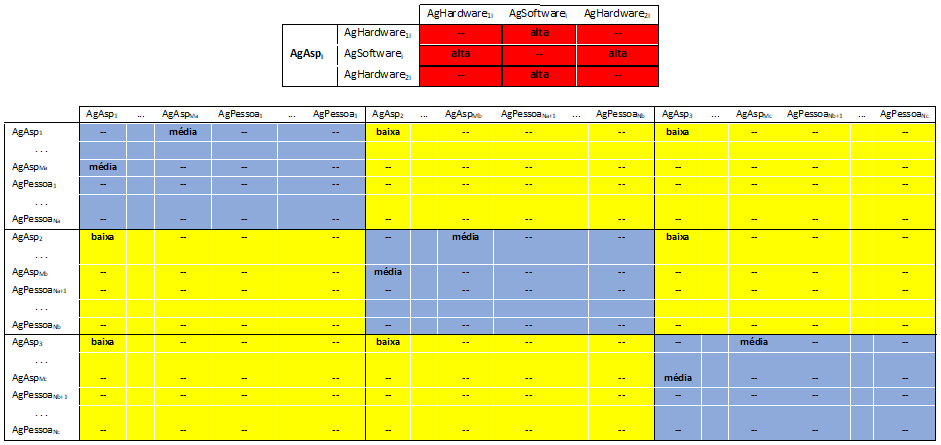
\includegraphics[width=\linewidth]{figuras/exp6-matriz-socio.png}
    }{
        \Fonte{Elaborado pelo autor}
    }   
\end{figure}

Na figura, a tabela menor indica que cada programa $AgAsp_i$ representa um aspirador $i$ do sistema técnico, ou seja, uma agregação de três programas na organização, isto é: $AgHardware_{1i}$, $AgHardware_{2i}$ e $AgSoftware_i$. A tabela maior informa uma baixa frequência de troca de mensagens entre os três coordenadores ($AgAsp_1$, $AgAsp_2$, $AgAsp3$) dos três grupos, uma frequência média entre os coordenadores de cada grupo e os seus coordenados ($AgAsp_1$, \ldots, $AgAsp_{Ma}$; $AgAsp_2$,  \ldots, $AgAsp_{Mb}$; $AgAsp_3$, \ldots, $AgAsp_{Mc}$), e que tanto coordenadores quanto seus coordenados não interagem com os programas representando as pessoas nas três zonas ($AgPessoa_1$, \ldots, $AgPessoa_{Na}$; $AgPessoa{Na+1}$, \ldots, $AgPessoa_{Nb}$; $AgPessoa_{Nb+1}$, \ldots, $AgPessoa_{Nc}$).

\subsubsection{Modelo C}

Conforme mencionado, o modelo $C$ foi alterado para acomodar os agentes coordenadores. Esta acomodação implicou na definição do comportamento de cada programa no papel $Controller$ coordenando um dos três grupos ($AgSoftware_1$, $AgSoftware_2$, $AgSoftware_3$), em uma alteração no modelo do comportamento dos outros programas no papel $Controller$ coordenados em um dos grupos ($AgSoftware_4$, \ldots, $AgSoftware_{Na}$, $AgSoftware_{Na+1}$, \ldots, $AgSoftware_{Nb}$, $AgSoftware_{Nb+1}$, \ldots, $AgSoftware_{Nc}$), e no protocolo de interação entre os programas.

Apesar do modelo $F$ não ter sido estendido, as informações sobre os estados do ambiente, percebidas pelos programas no papel \textit{Device} representando sensores, agregam informações a respeito de linhas divisórias entre as zonas compondo o ambiente. Assim, quando recebem estas informações, os programas no papel \textit{Controller} sendo coordenados e coordenadores evitam ultrapassar estas linhas. Entretanto, sempre que precisar, um coordenador pode requisitar a outro coordenador que envie alguns dos aspiradores para a sua zona. Neste caso o coordenador que recebeu a mensagem deve consultar seus coordenados visando descobrir aspiradores disponíveis, os quais devem assimilar a ideia e partir para a zona que requisitou ajuda. 

A Figura \ref{fig:exp6-protocolo} ilustra o protocolo de interação entre os programas no papel \textit{Controller}. A descrição do processo de comunicação considera um conjunto de seis estados possíveis, $Q = \{q_0, q_1, q_2, q_3, q_4, q_5\}$, em que o estado inicial foi representado por $q_0$. A figura supõe que o processo de conversação envolve um uma família de quatro conjuntos de programas $G = \{C, C_1, C_2, C_3\}$, ou seja: um conjunto de três programas coordenadores $C = \{AgAsp_1, AgAsp_2, AgAsp_3\}$, um conjunto de programas coordenados pelo coordenador $AgAsp_1$ da zona 1, isto é, $C_1 = \{AgAsp_4, \ldots, AgAsp_{Ma}\}$; um conjunto de programas coordenados pelo coordenador $AgAsp_2$ da zona 2, isto é, $C_2 = \{AgAsp_{Ma+1}, \ldots, AgAsp_{Mb}\}$; e um conjunto de programas coordenados pelo coordenador $AgAsp_3$ da zona 3, isto é, $C_3 = \{AgAsp_{Mb+1},  \ldots, AgAsp_{Mc}\}$.

\begin{figure}[h!]
    \centering
    \Caption{\label{fig:exp6-protocolo} Protocolo de interação entre os programas na organização.} 
    \UECEfig{}{
        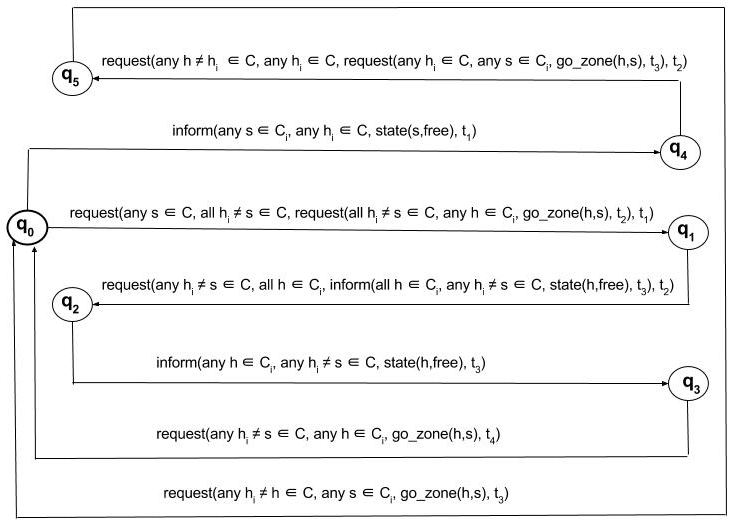
\includegraphics[width=10cm]{figuras/exp6-protocolo.png}
    }{
        \Fonte{Elaborado pelo autor}
    }   
\end{figure}

De acordo com a relação Communication, o protocolo de interação indica que os programas coordenadores se comunicam entre si e cada um com os programas por ele coordenados. As transições entre os estados $q_0-q_1$ e $q_4-q_5$ correspondem a solicitações envolvendo pelo menos três agentes (\textit{requests to request}), a transição entre os estados $q_1-q_2$ corresponde a uma pergunta (\textit{requests to inform}) envolvendo pelo menos dois agentes. O restante das transições corresponde às mensagens fundamentais para solicitar e informar (\textit{request e inform}) a um outro agente.

No instante $t_1$, a partir do estado inicial $q_0$, existem duas possibilidades de transição. Primeiro, qualquer coordenador $s$ no conjunto de coordenadores $C$ pode solicitar que cada coordenador $h_i$ no conjunto $C$ solicite que seus coordenados no conjunto $C_i$ se dirijam à zona do coordenador $s$. No instante $t_2$ o coordenador $h_i$ em C pergunta aos seus coordenados em $C_i$ a respeito de seus estados atuais. No instante $t_3$ um programa $h$ em $C_i$ que está livre, informa este fato ao seu coordenador $h_i$ em $C$. No instante $t_4$ o coordenador $h_i$ solicita que seu coordenado $h$ se dirija à zona do coordenador $s$, o qual solicitou esta ação no instante $t_1$.

Na segunda transição possível no instante $t_1$, um programa coordenado $h$ em um conjunto $C_i$ informa ao seu coordenador $h_i$ em $C$ que está livre. Sendo assim, se em $t_2$ algum coordenador $s$ em $C$ solicitar que o coordenador $h_i$ solicite que seus coordenados se dirijam à zona do coordenador $s$, então em $t_3$ o coordenador $h_i$ poderá solicitar imediatamente que $h$ no conjunto $C_i$ se dirija a zona de $s$, o qual solicitou esta ação no instante $t_2$, depois que $h$ informou que estava livre em $t_1$. 

A Figura \ref{fig:exp6-protocolo} omitiu a transição para o estão inicial $q_0$ na situação em que os programas coordenados e/ou coordenadores não enviam mensagens de retorno para as solicitações. Por exemplo, depois de $\epsilon$ unidades de tempo, contadas a partir do horário de início da conversação no instante $t_2 (time(t_2))$ até um tempo limite em que uma mensagem de retorno deve ser enviada no instante $t_3 (time(t_3))$, o protocolo deve transitar para o estado inicial, $\delta(q_2, time(t_3) – time(t_2) > \epsilon) = q_0$, em que os programas poderão iniciar novo processo de conversação.

\subsubsection{Objetos Emergentes}

Os objetos emergentes, resultantes das modificações realizadas neste experimento, são apresentados nesta subseção. As condições são as mesmas observadas no experimento anterior. Em cada teste serão três coordenadores, cada um responsável por uma zona. A quantidade de aspiradores por teste será variada da mesma forma que o experimento anterior. 

\begin{figure}[h!]
    \centering
    \Caption{\label{fig:exp6-perf-utilidade} Utilidade do sistema ni sexto experimento.} 
    \UECEfig{}{
        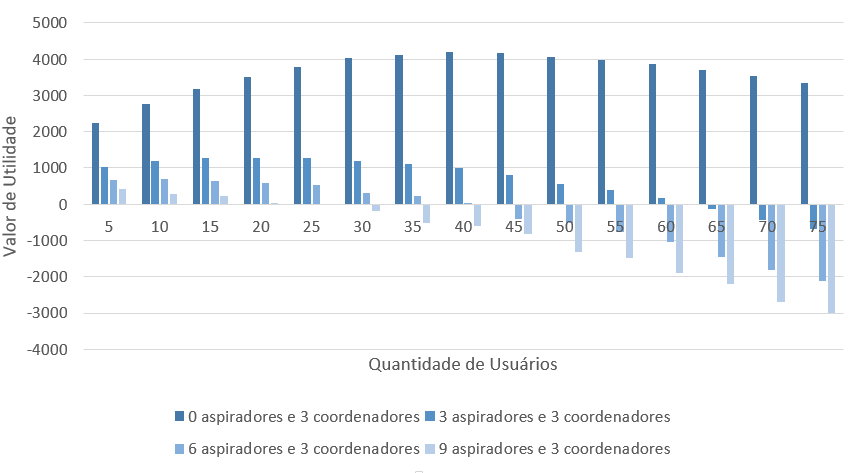
\includegraphics[width=10cm]{figuras/exp6-perf-utilidade}
    }{
        \Fonte{Elaborado pelo autor}
    }   
\end{figure}

Conforme podemos observar na Figura \ref{fig:exp6-perf-utilidade}, o desempenho do sistema foi bem inferior aos experimentos anteriores. Isso pode ser atribuído a um fator observado durante a execução. Como tanto os coordenadores quanto os aspiradores tem um espaço de movimento mais limitado, quando eles se posicionam em certas áreas, como nos cantos de suas respectivas zonas, eles tem menos opções de movimento, forçando o agente a seguir por uma direção que pode estar ocupada por algum usuário causando uma colisão com ele.  Como a função associada ao objetivo de evitar incomodar os usuários tem prioridade maior que as outras, o desempenho do sistema é bastante afetado. 

\begin{figure}[h!]
    \centering
    \Caption{\label{fig:exp6-perf-limpeza} Limpeza do ambiente no sexto experimento.} 
    \UECEfig{}{
        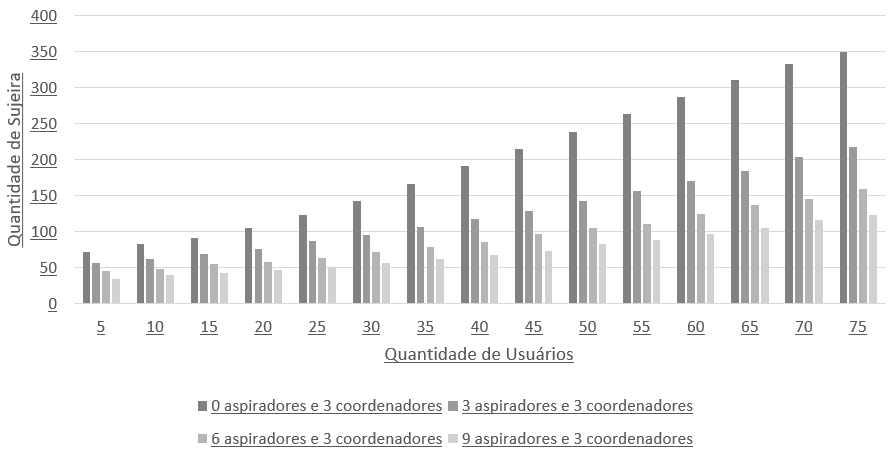
\includegraphics[width=10cm]{figuras/exp6-perf-limpeza}
    }{
        \Fonte{Elaborado pelo autor}
    }   
\end{figure}

Como podemos observar na Figura \ref{fig:exp6-perf-limpeza} acima, não é possível determinar uma diferença significativa entre o desempenho, relacionado a limpeza do ambiente, neste experimento e no observado na Figura \ref{fig:exp5-perf-limpeza}. Isso reforça a hipótese que a baixa performance do objetivo original está relacionada ao objetivo próximo $O_3$.

\section{Conclusão}
\label{sec:conclusao}

Neste capítulo foi mostrada a utilização do modelo \acrshort{fec}, elaborado no capítulo \ref{cap:abordagem}, para uma aplicação de sistemas de inteligência ambiental. Para construir o modelo dessa aplicação foi utilizada uma abordagem incremental, inserindo novos elementos no sistema a cada experimento e, consequentemente, aumentando sua complexidade. Cada um dos experimentos gera um conjunto de dados que são utilizados para avaliar o modelo construído para o sistema. 
A aplicação utilizada para o teste desse modelo tem como base o experimento clássico do aspirador de pó. Ela consiste em um sistema de inteligência ambiental onde um conjunto de agentes aspiradores de pó deve manter limpo um ambiente onde circulam grupos de pessoas. O objetivo desse sistema \acrshort{ami} é manter o ambiente limpo, minimizando os custos de energia e evitando atrapalhar as pessoas que estão passando.

No primeiro experimento realizado, a aplicação é simulada em um ambiente estático contendo apenas um agente aspirador. O intuito deste experimento é verificar se o modelo gerado para o agente aspirador é capaz de cumprir um dos objetivos da aplicação, limpar o ambiente, e validar o modelo de função gerado para esse objetivo. 

O segundo experimento também tem como objetivo observar o comportamento do agente e de seu modelo de função, mas dessa vez em um condições diferentes. O agente aspirador único é mantido na aplicação, porém, o ambiente de aplicação se torna dinâmico. Ou seja, o próprio programa de ambiente passa a inserir sujeira no ambiente. Além disso, o agente aspirador passa a apresentar falhas em seu atuador, perdendo sua característica determinística.

O terceiro experimento mantém as novas características do ambiente e do agente aspirador, e adiciona um novo elemento a simulação, o agente usuário. Neste experimento são observadas as medidas extraídas, a partir do modelo de função atualizado, da simulação em função da quantidade de pessoas no ambiente.

No quarto experimento passamos observar na simulação um ambiente contendo dois ou mais agentes aspiradores. Nele são extraídas medidas de três situações diferentes, na primeira são observadas as medidas em um ambiente contendo três aspiradores, na segunda passam a ser seis, e na terceira uma dúzia de aspiradores. 

O quinto experimento adiciona um novo agente a aplicação chamado agente coordenador. Com esse novo elemento a aplicação passa a apresentar características organizacionais mais complexas e novos elementos de cooperação. Isso gera mudanças mais profundas nos modelos de estrutura e comportamento definidos anteriormente, além de refletir nas medidas obtidas através do modelo de função.

Finalmente, o sexto experimento divide o ambiente da aplicação em três partes, onde cada uma dessas partes contém um agente coordenador que gerencia os aspiradores da sua zona.  Ambos os experimentos cinco e seis são realizados em condições semelhantes às do quarto experimento, examinando diferentes situações do ambiente em função da quantidade de pessoas que passam por ele. 

Para simplificar a apresentação dos experimentos, foram omitidas algumas características dos modelos \acrshort{fec} que se mantinham de um experimento para outro. Em cada experimento foram geradas duas distribuições, uma contendo as medidas associadas ao modelo de função, caracterizando o desempenho da aplicação em relação aos objetivos do sistema, e outra ilustrando especificamente a performance do sistema em relação a limpeza do ambiente. Essas distribuições extraídas da simulação permitem que o desenvolvedor possa observar características do sistema antes de iniciar sua implantação no mundo real.

Neste trabalho, os experimentos foram realizados com o objetivo de validar o modelo \acrshort{fec} proposto, cada um dos experimentos apresenta evoluções no modelo relacionadas a inserção de realidade no sistema \acrshort{ami}. As representações geradas na simulação a partir dos modelos foram aceitáveis. Expondo características do sistema que não poderiam ser observadas antes de sua construção. Isso pode ser observado principalmente nos três últimos experimentos, onde podemos notar que as mudanças de comportamento e estrutura propostas no sistema não são capazes de gerar ganhos significativos de acordo com o modelo de Função adotado.


%%%%%%%%%%%%%%%%%%%%%%%%%%%%%%%%%%%%%%%%%

\begin{comment}

        \begin{algorithm}[h!]
            %\SetSpacedAlgorithm
            \caption{\label{alg:decision-function} Descrição parcial da função tomada de decisão de um agente reativo.}
            %\Entrada{$p^k$ em S}
            %\Saida{$a^k$ em A}
            função ação ($p^k$ em S) retorna $a^k$ em A\\
            \Inicio{
                \ldots\\
                \textbf{se} $p^k$ = obstaculo \textbf{então} \textbf{retornar} $a^k$ = aspirar\;
                \textbf{senão se} $p^k$ = obstaculo \textbf{então} \textbf{retornar} $a^k$ = rotacionar $90^\circ$ esquerda\;
                \textbf{senão se} $p^k$ = limpo \textbf{então} \textbf{retornar} $a^k$ = frente\;
                \ldots\\
            }
        \end{algorithm}


    \begin{table}[h!]   
    \centering
    \Caption{\label{tab:modelF-exp1} Definição dos termos envolvidos no esqueleto do programa de agente.}
    \UECEtab{}{
        \begin{tabular}{| p{4cm} | p{10cm}|}
        \hline
        $S = \{s_1, s_2, \ldots \}$ & Estados do ambiente –- em qualquer instante $k$ o sensor do aspirador disponibiliza um estado $s^k$ consistindo de uma grade menor, contida na grade $32\times32$ \textit{patches} que representa o local, de tamanho $3\times3$ \textit{patches}, ou seja, o conjunto de estados do ambiente é formado por todas as grades desse tamanho, em que cada \textit{patch} pode representar uma parte limpa (branco) ou suja (cinza) do local, ou a presença de um obstáculo (marrom) na parte;\\ \hline
        
        $A = \{a_1, a_2, \ldots \}$ & Capacidade efetuadora -– em qualquer instante $k$ o atuador do aspirador consegue executar uma ação $a^k$ que pode ser: locomover-se do \textit{patch} em que o aspirador está para outro \textit{patch}, em qualquer direção (norte, sul, leste, oeste), ou limpar o \textit{patch} em que o aspirador está (aspirar);      \\ \hline
        
        ação:$S^*  \rightarrow A \}$ & Comportamento -– função para seleção de ações em $A$ adequadas aos estados em $S$, ou seja, o aspirador deve aspirar em \textit{patches} cinza, e deve mudar para um \textit{patch} vizinho que seja cinza se estiver em um \textit{patch} branco;   \\ \hline
        
        amb: $S\times A \rightarrow S$ & Comportamento (determinístico) ambiente –- função para mudança de estados do ambiente de acordo com as ações executadas pelo agente – se o aspirador limpar em um \textit{patch} cinza então este deve mudar para branco, e se o aspirador seguir de um \textit{patch} para outro em uma determinada direção então mudar posição do agente para este outro \textit{patch};   \\ \hline
        
        AgentAmI & Um programa de agente implementando concretamente em linguagem NetLogo a função ação de um agente aspirador; \\ \hline
        
        Amb & Um programa ambiente implementando concretamente em linguagem NetLogo a função amb; \\ \hline
         
        $\Omega$ & Um conjunto formado por todas as grades de tamanho $32 \times 32$ \textit{patches}, diferentes quanto a quantidade de \textit{patches} do tipo cinza;  \\ \hline
        
        $Cenario_i \in \Omega$ & Uma grade de tamanho $32 \times 32$ \textit{patches}, os quais podem ser do tipo branco, cinza ou marrom; \\ \hline
    
        $Cenario_i \in P(\Omega)$ & Um subconjunto formado por $10 (N_{Cenarios)}$ grades de $32 \times 32$ \textit{patches}, os quais podem ser do tipo branco, cinza ou marrom; \\ \hline
        
        $h(Cenario_i) \in (S\times A)^{Nint}$ & Uma história formada por 100 ($NInt$) de $AgentAmI$ em $Amb$ correspondente ao $Cenario_i \in \Omega$; \\ \hline
        
        $Ep^k(h(Cenario_i)) \in (S\times A)$ & Um episódio na interação k, $k \leq 10$, da história de $AgentAmI$ em $Amb$ correspondente ao caso $Cenarioi \in \Omega$; \\ \hline
        
        $H(Cenario_i)) \in P((S\times A)^{Nint})$ & Um conjunto de 10 histórias de comprimento 100 de $AgentAmI$ em $Amb$; \\ \hline
        
        \end{tabular}
    }{
    \Fonte{Elaborado pelo autor}
}
\end{table}




Como estudo de caso para a abordagem que propomos neste trabalho, utilizaremos quatro cenários distintos. Todos os cenários tem como os origem o exemplo clássico do aspirador de pó, que já foi utilizado em diferentes contextos nesse trabalho. Cada um desses cenários busca extrair um tipo diferente de informação dos agentes executados, de acordo com as diferentes níveis que desejamos observar (ambientes mais simples, ou mais complexos).

Em um primeiro cenário, estaremos observando o comportamento de um único agente aspirador em um ambiente parcialmente observável. Nesse ambiente serão extraídas informações quanto a performance do agente (desperdício de energia e limpeza do ambiente). No segundo cenário, adicionaremos um conjunto de agentes ao mesmo ambiente. No entanto, eles não serão capazes de se comunicar, a intenção é observar o impacto no ambiente das ações desordenadas desses agentes, medindo a eficiência dessas ações. No terceiro e quarto cenários, também utilizaremos um time de agentes para aspirar um ambiente, mas serão utilizadas duas estrategias de comunicação distintas em cada um desses cenários. 

Ao fim desses testes, vamos comparar o grau de eficiência de cada um dos cenários (Limpeza $\times$ Desperdício de energia). Cada um desses cenários será construído na plataforma de simulação de agentes NetLogo \cite{wilensky1999netlogo}. A razão para a escolha dessa plataforma é alta simplicidade em representar os agentes, facilitando a construção de ambientes complexos em curto espaço de tempo. 

NelLogo é uma linguagem de programação com atributos multi-agentes. Ela possui capacidades que a tornam muito poderosa, tanto para produzir quanto para visualizar simulações de \acrlong{sma}. NetLogo é implementada em Java, e possui um código compacto e simples de se compreender, tornando-a ideal para demonstrar ideias complexas de forma sucinta. E além disso ela permite que os usuários adicionem extensões para a linguagem, criando novos comandos escritos em Java \cite{teahan2010artificial}.

 Em NetLogo existem quatro tipos de agentes inteligentes, \textit{patches}, \textit{turtles}, \textit{links}, e \textit{observer}. \textit{Turtles} são os agentes com capacidade de movimentar pelo ambiente e interagir ele. \textit{Patches} são agentes que representam o ambiente por onde os \textit{turtles} caminham. Em um ambiente bidimensional os \textit{patches} são representados por um \textit{grid}, onde cada célula contem um \textit{patch}. Os agentes \textit{links} não possuem uma representação visual, mas são responsáveis pela comunicação entre dois ou mais agentes \textit{turtles}. O agente \textit{observer} também não possui uma representação visual, mas ele é responsável por enviar comandos a todos os outros agentes e monitorar suas atividades. O código apresentado abaixo ilustra a estrategia de movimentação de um agente aspirador de pó.

\lstinputlisting[caption=Codigo em em NetLogo para movimentação do agente inteligente, frame=single, language=NetLogo, basicstyle=\tiny]{codigos/inteligent_agent.nlogo}

Na estrategia apresentada acima o comando \textit{ask turtles}, pede para que todos os agentes \textit{turtles} executem as seguintes instruções. Primeiro o agente (representado por um circulo vermelho) verifica se ele pode se mover uma casa a frente, caso exista um obstaculo a frente (\textit{patch} com cor marrom) ele deve virar em uma direção randômica. Mas se o caminho estiver livre ele da um passo a frente e examina as casas ao redor, verificando se existe sujeira em algum \textit{patch} (cor cinza) em uma distancia menor ou igual a três. Se existir ele vira para a direção da sujeira mais próxima, e reinicia o \textit{loop} de movimento. A Figura \ref{fig:exemplo-netlogo} ilustra a ação desse agente. 


\begin{figure}[h!]
    \centering
    \Caption{\label{fig:exemplo-netlogo} Exemplo de um agente aspirador de pó em um ambiente NetLogo} 
    \UECEfig{}{
        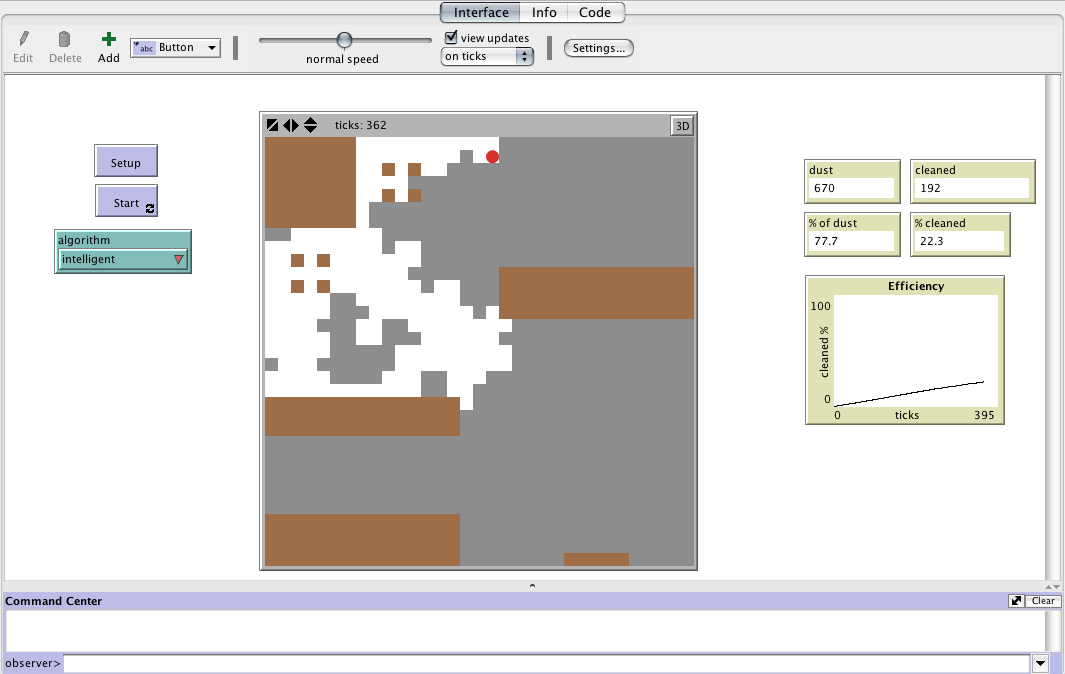
\includegraphics[width=8cm]{figuras/exemplo-netlogo}
    }{
        \Fonte{Elaborado pelo autor}
    }   
\end{figure}


\section{Cronograma}
O cronograma para a finalização do trabalho é o seguinte:

\begin{quadro}[h!]  
    \centering
    \Caption{\label{qua:cronograma} Cronograma.}
    \UECEqua{}{
        \begin{tabular}{|c|c|c|c|c|}
            \hline
            & Março & Abril & Maio & Junho \\
            \hline
            Implementação   & X & X & X & -\\
            \hline
            Testes          & - & X & X & -\\
            \hline
            Artigos         & - & X & X & X \\
            \hline
            Finalização     & - & - & X & X \\
            \hline
            Apresentação    & - & - & - & X \\
            \hline
        \end{tabular}
    }{
        \Fonte{Elaborado pelo autor}
    }
\end{quadro}

\end{comment}